\section{Considerações iniciais}

O processo de manipular imagens para que elas se tornem mais satisfatórias para um
determinado objetivo depende do domínio de aplicação. Ou seja, não existe uma teoria geral para melhorar qualquer imagem \cite{Gonzalez2007}; um método que processa melhor uma imagem bem definida por suas cores difere do processamento de imagens texturizadas, às quais um processamento sobre a intensidade dos pixels da imagem --- como uma operação de borramento --- pode ocasionar perda da textura. Assim, justifica-se a exploração de um vasto número de métodos de processamento de imagens e bases.

Neste capítulo oito métodos de processamento de imagens são utilizados com o fim de obter imagens artificiais para sobreamostrar classes minoritárias em problemas de classificação, rebalanceando as bases de imagens antes da extração de características. Isso é realizado com dois propósitos: 1) para compensar a baixa disponibilidade de exemplos de uma determinada classe, e 2) permitir a extração de informações antes não disponíveis nas imagens originais por meio da combinação ou perturbação das imagens de entrada.

Dada a quantidade de imagens necessárias para rebalancear a base original, são geradas novas imagens a partir de um conjunto de métodos. Como demonstrado na Figura~\ref{fig:escolha}, dado o conjunto de treinamento da classe (ou classes) com menor número total de imagens, é realizado o rebalanceamento ao aplicar os métodos descritos neste capítulo. Posteriormente, essas imagens resultantes têm suas características extraídas e são utilizadas no treinamento da classe minoritária.

\begin{figure}[!htbp]
  \begin{center}
    \includegraphics[width=0.7\linewidth]{\detokenize {figuras/rebalance.pdf}}
  \end{center}
  \caption[Geração artificial da classe minoritária para rebalancear a base de imagens. Para cada imagem necessária para igualar o número de imagens da base, $1 \leq n \leq 16$ imagens originais são dadas como entrada para uma operação de geração artificial. A nova imagem é utilizada como treinamento da base.]{Geração artificial da classe minoritária para rebalancear a base de imagens. Para cada imagem necessária para igualar o número de imagens da base, $1 \leq n \leq 16$ imagens originais são dadas como entrada para uma operação de geração artificial. A nova imagem é utilizada como treinamento da base. \\ \textit{Fonte: Elaborado pela autora.}}
  \label{fig:escolha}
\end{figure}

Os resultados encontrados ao rebalancear classes a partir da geração de imagens artificiais são também apresentados neste capítulo. Para cada experimento realizado, são descritos: o protocolo utilizado (i.e. base de imagens, os métodos de conversão para escala de cinza e extração de características), os resultados encontrados e a discussão da relevância de tais resultados.

Foram realizados diversos experimentos direcionados a explorar o rebalanceamento com os métodos de processamento, com o objetivo de melhorar a acurácia da classificação de bases de imagens. Como entrada são utilizadas imagens provenientes de diversas coleções disponíveis na literatura. Como resultado, são calculadas medidas estatísticas da classificação dessas bases de imagens após o rebalanceamento destas. Tal processamento é realizado antes da extração de características, e portanto no campo visual. Espera-se que os resultados encontrados proporcionem melhoras na etapa subsequente de classificação.

\section{Métodos para geração de imagens artificiais}

Os métodos de geração artificial para o rebalanceamento de classes de imagens são descritos nesta seção. Os experimentos, posteriormente destacados na Seção~\ref{sec:resultados-geracao}, foram realizados utilizando as operações de: \emph{borramento}; \emph{mistura ponderada}; \textit{aguçamento}; \emph{composição}; \emph{mistura limiarizada}; \emph{mistura saliente}; \emph{SMOTE visual}; e \emph{adição de ruído}.

%%%%%%%%%%%%%%%%%%%%%%%%%%%%%%%%%%%%%%%%%%%%%%%%%%%%%%%%%%%%%%%%%%%%%%%%%%%%%%%%
\subsection{Borramento}

Também conhecido como suavização, o \emph{borramento} é uma operação de processamento comumente utilizada com o objetivo de filtrar uma imagem, removendo ruídos e detalhes não relevantes. Normalmente esse tipo de filtragem provoca também um certo borramento das bordas, como pôde ser observado anteriormente na Figura~\ref{fig:blur}. Esse comportamento não é esperado quando queremos gerar novas imagens, pois informações relevantes podem ser removidas. Com o intuito de preservar as bordas, a operação de borramento \textbf{filtro bilateral} pode ser utilizada. Ela substitui o valor do pixel $I(x,y)$ pela média dos pixels vizinhos de intensidade similar \cite{Tomasi1998}. Ou seja, é uma média ponderada das intensidades que considera a diferença dos valores entre vizinhos para preservar bordas. Assim, para um pixel influenciar outro, deve estar próximo no espaço de coordenadas e possuir intensidade similar. O Algoritmo~\ref{alg:blur} descreve os passos desse filtro na sua versão mais simples, de força bruta. Considere $W$ o termo de normalização, e $G$ o filtro de Gaussianas. A Figura~\ref{fig:gen:blur} exemplifica o seu funcionamento: à esquerda está demonstrada a imagem original e à direita a imagem borrada.

\begin{algorithm}[!htbp]
  \caption{Geração artificial: \emph{borramento} com filtro bilateral}
  \label{alg:blur}
  \SetAlgoLined
  \Entrada{
  \begin{itemize}
    \item[] Imagem colorida $I_{original}$ em formato RGB
    % \item[] Diâmetro $d$ de vizinhança de pixels
    \item[] Sigma do espaço de cor $\sigma_{range}$
    \item[] Sigma do espaço de coordenadas $\sigma_{spatial}$
  \end{itemize}
  }
  \Saida{
  \begin{itemize}
    \item[] Imagem borrada $I_{borrada}$
  \end{itemize}
  }
  \ParaCada{pixel $(x,y)$}{
    $I_{borrada}(x,y) \gets 0$\;
    $W(x,y) \gets 0$\;

    \ParaCada{pixel $(i,j)$}{
      $w \gets G_{\sigma_{spatial}} (\lVert(x,y) - (i,j)\rVert) G_{\sigma_{range}} (\lvert I_{original}(x,y) - I_{original}(i,j) \rvert) $\;
      $I_{borrada}(x,y) \gets I_{borrada}(x,y) + w I_{original}(i,j)$\;
      $W(x,y) \gets W(x,y) + w$\;
    }
    $I_{borrada}(x,y) \gets I_{borrada}(x,y) / W(x,y)$\;
  }
\end{algorithm}

\begin{figure}[!htbp]
  \begin{center}
    \subfloat[Original]{
      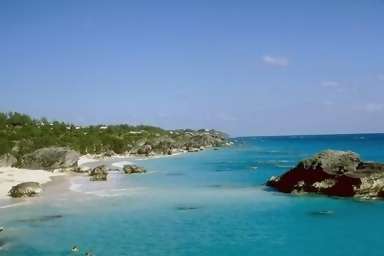
\includegraphics[width=.48\linewidth]{\detokenize{figuras/geracao/blur-a.png}}
    }
    \subfloat[Imagem artificial]{
      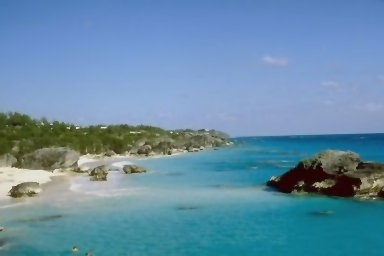
\includegraphics[width=.48\linewidth]{\detokenize{figuras/geracao/blur-b.png}}
    }
  \end{center}
  \caption[Geração artificial utilizando \emph{borramento} com filtro bilateral. A imagem (b) possui detalhes borrados, porém preservando as bordas.]{Geração artificial utilizando \emph{borramento} com filtro bilateral. A imagem (b) possui detalhes borrados, porém preservando as bordas. \\ \textit{Fonte:~Elaborado pela autora.}}
  \label{fig:gen:blur}
\end{figure}

\begin{description}
  \item[Parâmetros e suas variações] Conforme descrito no Algoritmo~\ref{alg:blur}, os parâmetros para essa geração são: o $\sigma_{range}$ do espaço de cor e o $\sigma_{spatial}$ do espaço de coordenadas. Esses parâmetros dependem das propriedades das imagens e dos resultados pretendidos. Quanto maior o $\sigma_{range}$, mais próximo da convolução Gaussiana e assim ocorre o borramento de intensidades mais distintas. Já o $\sigma_{spatial}$ controla o tamanho da vizinhança. Dessa forma, esses valores são escolhidos arbitrariamente para cada aplicação específica \cite{Tomasi1998}. Como o nosso objetivo com a geração das imagens não foi especializar no comportamento de uma classe de imagens, um valor foi escolhido aleatoriamente, e a partir dele os parâmetros de entrada foram definidos.

  \item[Limitações] Esse filtro tende a remover texturas e criar novos contornos. Dependendo dos valores, pode gerar uma imagem ``cartoonizada''.

  \item[Métodos relacionados] São diversos os métodos de borramento descritos na literatura, como a filtragem Gaussiana e de médias.
\end{description}
%%%%%%%%%%%%%%%%%%%%%%%%%%%%%%%%%%%%%%%%%%%%%%%%%%%%%%%%%%%%%%%%%%%%%%%%%%%%%%%%
\FloatBarrier
\subsection{Aguçamento}

Diferente da suavização, o processamento de \emph{aguçamento} procura enfatizar as transições de intensidade. Um método bem conhecido para atingir tal objetivo é o \textit{unsharp mask}. Ele borra a imagem, subtrai a imagem borrada da original e adiciona essa diferença na imagem original, dado um peso $k$ (ver Algoritmo \ref{alg:unsharp}). A imagem resultante, ilustrada na Figura~\ref{fig:gen:unsharp}, é uma versão realçada da imagem original. Isso porque adiciona à imagem justamente o que é removido com um filtro de suavização.

\begin{algorithm}[!htbp]
  \caption{Geração artificial: \emph{aguçamento}}
  \label{alg:unsharp}
  \SetAlgoLined
  \Entrada{
  \begin{itemize}
    \item[] Imagem colorida $I_{\textit{original}}$ em formato RGB
  \end{itemize}
  }
  \Saida{
  \begin{itemize}
    \item[] Imagem aguçada $I_{\textit{aguçada}}$\\
  \end{itemize}
  }
  $I_{\textit{borrada}} \gets \textit{filtro de suavização}(I_{\textit{original}})$

  \ParaCada{canal de cor em $I_{\textit{original}}$}{
    \ParaCada{pixel $(x,y)$ em $I_{\textit{original}}$}{
    $I_{\textit{diferença}} \gets I_{\textit{original}}(x,y) - I_{\textit{borrada}}(x,y)$\;
    $I_{\textit{aguçada}}(x,y) \gets I_{\textit{original}}(x,y) + k \times I_{\textit{diferença}}$\;
    }
  }
\end{algorithm}

\begin{figure}[!htbp]
  \begin{center}
    \subfloat[Original]{
      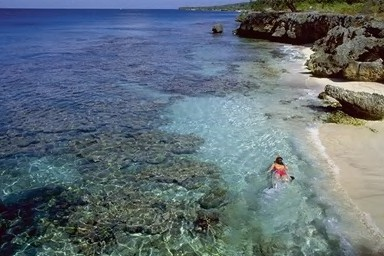
\includegraphics[width=.48\linewidth]{\detokenize{figuras/geracao/unsharp-a.png}}
    }
    \subfloat[Imagem artificial]{
      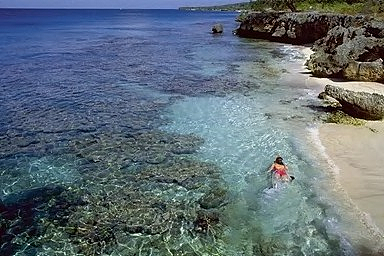
\includegraphics[width=.48\linewidth]{\detokenize{figuras/geracao/unsharp-b.png}}
    }
  \end{center}
  \caption[Geração artificial utilizando \textit{unsharp masking}. A imagem resultante (b) apresenta saliência nas transições de intensidade.]{Geração artificial utilizando \textit{unsharp masking}. A imagem resultante (b) apresenta saliência nas transições de intensidade. \\ \textit{Fonte:~Elaborado pela autora.}}
  \label{fig:gen:unsharp}
\end{figure}

\begin{description}
  \item[Parâmetros e suas variações] Pode-se variar o parâmetro $k$ de forma a ponderar a soma dessa diferença. Para a geração das imagens da classe minoritária, foi utilizado $k = 1$.

  \item[Limitações] É possível que existam pixels com valor negativo no resultado final. Isso pode causar o aparecimento de uma áurea em volta das bordas, efeito não desejado \cite{Gonzalez2007}.

  \item[Métodos relacionados] Outros algoritmos conhecidos para o aguçamento de imagens são: utilizar primeira derivada (gradiente), ou a segunda derivada da imagem (Laplaciano).
\end{description}
%%%%%%%%%%%%%%%%%%%%%%%%%%%%%%%%%%%%%%%%%%%%%%%%%%%%%%%%%%%%%%%%%%%%%%%%%%%%%%%%
\FloatBarrier
\subsection{Adição de ruído}

O ruído de Poisson ocorre na contagem de fótons de dispositivos ópticos. Ele segue a distribuição de Poisson, que representa o número de ocorrências de um evento em um dado instante de tempo \cite{Knuth1997}. O efeito da \emph{adição de ruído} pode ser visto na Figura~\ref{fig:gen:noise}.

\begin{figure}[!htbp]
  \begin{center}
    \subfloat[Original]{
      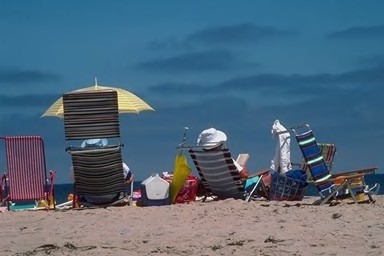
\includegraphics[width=.48\linewidth]{\detokenize{figuras/geracao/noise-a.png}}
    }
    \subfloat[Imagem artificial]{
      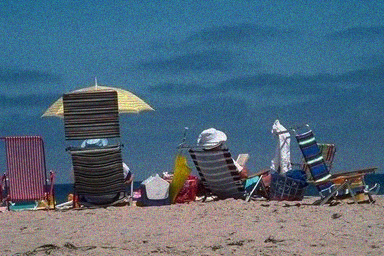
\includegraphics[width=.48\linewidth]{\detokenize{figuras/geracao/noise-b.png}}
    }
  \end{center}
  \caption[Geração artificial utilizando \emph{adição de ruído} de Poisson. Regiões claras de (b) apresentam mais ruído que as regiões escuras.]{Geração artificial utilizando \emph{adição de ruído} de Poisson. Regiões claras de (b) apresentam mais ruído que as regiões escuras. \\ \textit{Fonte:~Elaborado pela autora.}}
  \label{fig:gen:noise}
\end{figure}

% A distribuição de Poisson segue a equação:
% \begin{equation}
% $P_\mu)(n) = (e^(-\mu)\mu^(n))/(n!), n >= 0$
% \end{equation}

Uma possível implementação para encontrar os valores de Poisson foi desenvolvida por \citeonline{Knuth1997} e pode ser vista no Algoritmo~\ref{alg:noise}. A diferença do cálculo da distribuição de Poisson para sua adição em uma imagem é que, para calcular o valor de ruído em um pixel, esse pixel é considerado a média dessa distribuição. Ou seja, $\mu \equiv I_{original}(x,y)$. Para intensidades próximas a zero, o limite será $L \approx 1$ e, portanto, a probabilidade $p$ estará muito próxima do limite e o contador $k$ terá um valor baixo. Dessa forma, para intensidades escuras haverá pouco ruído. Por outro lado, em intensidades próximas a 255, $p \approx 0$. Assim, são necessárias muitas interações até $p > L$ e maior será a intensidade resultante $k-1$.

\begin{algorithm}[!htbp]
  \caption{Geração artificial: \emph{adição de ruído} de Poisson}
  \label{alg:noise}
  \SetAlgoLined
  \Entrada{
  \begin{itemize}
    \item[] Imagem colorida $I_{original}$ em formato RGB
  \end{itemize}
  }
  \Saida{
  \begin{itemize}
    \item[] Imagem gerada $I_{gerada}$\\
  \end{itemize}
  }

  \ParaCada{canal de cor em $I_{\textit{original}}$}{
    \ParaCada{pixel $(x,y)$ em $I_{\textit{original}}$}{
    $L \gets exp(-I_{original}(x,y))$\;
    $p \gets 1$\;
    $k \gets 0$\;
    \DoWhile{$p > L$}{
    $k \gets k + 1$\;
    $p \gets p \times \textit{número aleatório uniforme entre 0 e 1}$\;
    }
    $I_{ruidosa}(x,y) \gets k - 1$\;
    }
  }
\end{algorithm}

\begin{description}
  \item[Parâmetros e suas variações] Para a adição desse ruído em uma imagem, não é fornecido nenhum parâmetro. O ruído é calculado para cada pixel.
  \item[Limitações] A adição de ruído é normalmente indesejável. Porém, a utilizamos para englobar um processamento de imagens que, de certa forma, se contrapõe ao \emph{borramento}.
  \item[Métodos relacionados] Esse método está relacionado com diversos outros ruídos, como o sal e pimenta, por exemplo.
\end{description}
%%%%%%%%%%%%%%%%%%%%%%%%%%%%%%%%%%%%%%%%%%%%%%%%%%%%%%%%%%%%%%%%%%%%%%%%%%%%%%%%
\FloatBarrier
\subsection{\emph{SMOTE visual}}

Conforme visto na Seção \ref{sec:smote}, o SMOTE é um método de rebalanceamento aplicado após a extração de características. É proposta uma alternativa, chamada de \emph{SMOTE visual}, onde imita-se o funcionamento do SMOTE, porém no nível de pixels. A diferença é que não é feito entre as imagens mais próximas, mas sim entre duas imagens escolhidas de forma aleatória do conjunto de treinamento da classe minoritária.

Para cada pixel é calculada a diferença entre as duas imagens. Essa diferença é então multiplicada por um número aleatório no intervalo $[0-1]$ e adicionada
na imagem original (ver Algoritmo~\ref{alg:smotevisual}). O efeito que esse processamento causa na imagem pode ser visualizado na Figura~\ref{fig:gen:smotevisual}.

\begin{algorithm}[!htbp]
  \caption{Geração artificial: \emph{SMOTE visual}}
  \label{alg:smotevisual}
  \SetAlgoLined
  \Entrada{
  \begin{itemize}
    \item[] Imagem colorida $I_{original}$ em formato RGB
    \item[] Imagem colorida $I_{\textit{segunda\_original}}$ em formato RGB
  \end{itemize}
  }

  \Saida{
  \begin{itemize}
    \item[] Imagem gerada $I_{gerada}$\\
  \end{itemize}
  }

  \ParaCada{canal de cor em $I_{\textit{original}}$}{
    \ParaCada{pixel $(x,y)$ em $I_{\textit{original}}$} {
    $\textit{diferença} \gets I_{original}(x,y) - I_{\textit{segunda\_original}}(x,y)$\;
    $\text{gap} \gets \textit{número aleatório entre 0 e 1}$\;
    $I_{gerada}(x,y) \gets I_{original}(x,y) + gap \times \textit{diferença}$\;
    }

    $\textit{mínimo} \gets \textit{menor valor}(I_{gerada})$\;

    $\textit{máximo} \gets \textit{maior valor}(I_{gerada})$\;

    \ParaCada{pixel $(x,y)$ em $I_{\textit{original}}$} {
    $I_{gerada}(x,y) \gets I_{gerada}(x,y) - \textit{mínimo}$\;
    }

    \ParaCada{pixel $(x,y)$ em $I_{\textit{original}}$} {
    $I_{gerada}(x,y) \gets I_{gerada}(x,y) \times (255/(\textit{máximo} - \textit{mínimo}))$\;
    }
  }
\end{algorithm}

\begin{figure}[!htbp]
  \begin{center}
    \subfloat[Original]{
      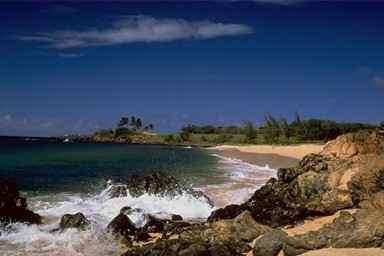
\includegraphics[height=4cm,keepaspectratio]{\detokenize{figuras/geracao/smote-a.png}}
    }
    \subfloat[Original]{
      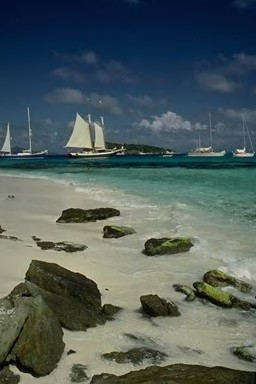
\includegraphics[height=4cm,keepaspectratio]{\detokenize{figuras/geracao/smote-b.png}}
    }
    \subfloat[Imagem artificial]{
      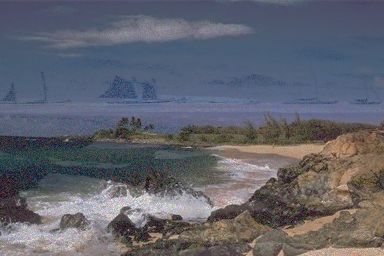
\includegraphics[height=4cm,keepaspectratio]{\detokenize{figuras/geracao/smote-c.png}}
    }
  \end{center}
  \caption[Geração artificial utilizando o método SMOTE no espaço visual. É possível notar a sobreposição de uma ``sombra'' da Figura (b) em (a). A imagem (b) foi redimensionada para as dimensões originais da imagem (a).]{Geração artificial utilizando o método SMOTE no espaço visual. É possível notar a sobreposição de uma ``sombra'' da Figura (b) em (a). A imagem (b) foi redimensionada para as dimensões originais da imagem (a).\\ \textit{Fonte:~Elaborado pela autora.}}
  \label{fig:gen:smotevisual}
\end{figure}

\begin{description}
  \item[Limitações] Esse método adiciona texturas e bordas que não estavam originalmente nas imagens.

  \item[Métodos relacionados] Esse método é visualmente parecido com o de \emph{mistura ponderada}, apresentado na próxima seção.
\end{description}
%%%%%%%%%%%%%%%%%%%%%%%%%%%%%%%%%%%%%%%%%%%%%%%%%%%%%%%%%%%%%%%%%%%%%%%%%%%%%%%%
\FloatBarrier
\subsection{Mistura ponderada}

Essa geração calcula a soma ponderada de duas imagens, de acordo com o
Algoritmo~\ref{alg:blend}. O efeito dessa mistura pode ser visto na Figura~\ref{fig:gen:blend}, onde dadas duas imagens como entrada, a imagem de saída corresponde à soma delas.

\begin{algorithm}[!htbp]
  \caption{Geração artificial: \emph{mistura ponderada}}
  \label{alg:blend}
  \SetAlgoLined
  \Entrada{
    \begin{itemize}
      \item[] Primeira imagem colorida $I$ em formato RGB
      \item[] Segunda imagem colorida $I_2$ em formato RGB
    \end{itemize}
  }
  \Saida{Imagem gerada $I_{gerada}$}

  {$\alpha \gets \textit{número aleatório entre 10 e 90}$\;}
  {$\beta \gets 100 - \alpha$\;}

  \ParaCada{pixel $(x,y)$} {
  $I_{gerada}(x,y) \gets \beta I(x,y) + \alpha I_2(x,y)$\;
  }
\end{algorithm}

\begin{figure}[!htbp]
  \begin{center}
    \subfloat[Original]{
      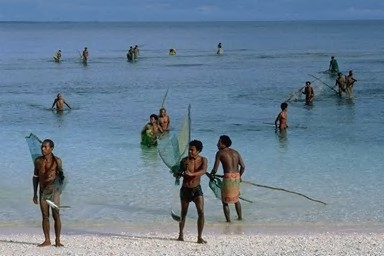
\includegraphics[width=.32\linewidth]{\detokenize{figuras/geracao/blend-a.png}}
    }
    \subfloat[Original]{
      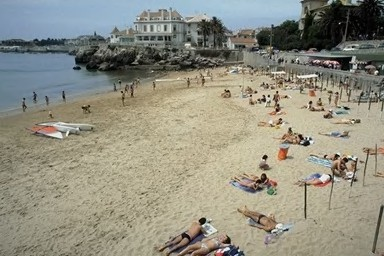
\includegraphics[width=.32\linewidth]{\detokenize{figuras/geracao/blend-b.png}}
    }
    \subfloat[Imagem artificial]{
      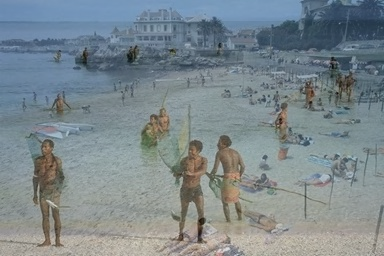
\includegraphics[width=.32\linewidth]{\detokenize{figuras/geracao/blend-c.png}}
    }
  \end{center}
  \caption[Geração artificial utilizando uma \emph{mistura ponderada} de duas imagens. A imagem (c) representa a mistura de (a) e (b).]{Geração artificial utilizando uma \emph{mistura ponderada} de duas imagens. A imagem (c) representa a mistura de (a) e (b). \\ \textit{Fonte:~Elaborado pela autora.}}
  \label{fig:gen:blend}
\end{figure}

\begin{description}
  \item[Parâmetros e suas variações] Os parâmetros $\alpha$ e $\beta$ são escolhidos de forma aleatória. Um valor entre 10\% e 90\% é escolhido para $\alpha$; e $\beta$ equivale ao valor restante para completar 100\%.

  \item[Limitações] Assim como todas as gerações artificiais que envolvem a mistura de imagens, efeitos são adicionados às imagens originais. Dependendo da combinação dos métodos de descrição, quantização e classificação, isso pode piorar a acurácia da classificação.

  \item[Métodos relacionados] É um método de combinação de imagens primitivo. Algoritmos similares são muito mais complexos, como os de limiares e saliência descritos a seguir.
\end{description}
%%%%%%%%%%%%%%%%%%%%%%%%%%%%%%%%%%%%%%%%%%%%%%%%%%%%%%%%%%%%%%%%%%%%%%%%%%%%%%%%
\FloatBarrier
\subsection{Mistura limiarizada}

A \emph{mistura limiarizada} é uma composição do fundo (\textit{background}) de uma imagem e do objeto da cena (\textit{foreground}) de outra imagem. A Figura~\ref{fig:gen:threshold} mostra a mistura dos \textit{thresholds} de duas imagens originais para compor uma nova imagem. O Algoritmo~\ref{alg:threshold} descreve as operações necessárias para realizar tal processamento, que utiliza OTSU para encontrar o \textit{foreground} da primeira imagem. Após, operações morfológicas são realizadas para melhorar a definição dos limiares.

\begin{figure}[!htbp]
  \begin{center}
    \subfloat[Original]{
      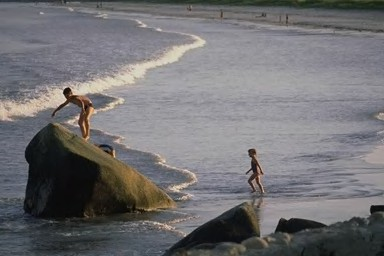
\includegraphics[width=.32\linewidth]{\detokenize{figuras/geracao/threshold-a.png}}
    }
    \subfloat[Original]{
      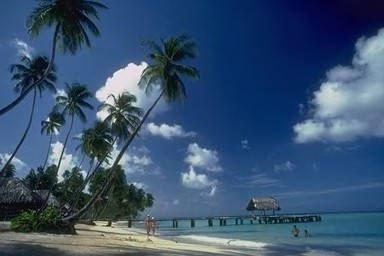
\includegraphics[width=.32\linewidth]{\detokenize{figuras/geracao/threshold-b.png}}
    }
    \subfloat[Imagem artificial]{
      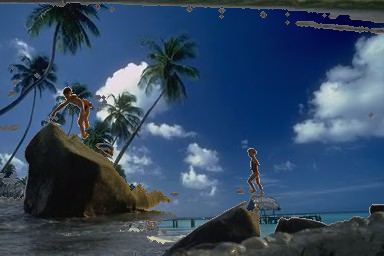
\includegraphics[width=.32\linewidth]{\detokenize{figuras/geracao/threshold-c.png}}
    }
  \end{center}
  \caption[Geração artificial utilizando uma \emph{mistura limiarizada} de duas imagens. A imagem resultante (c) é uma composição do \textit{foreground} da primeira imagem sobre o \textit{background} da segunda.]{Geração artificial utilizando uma \emph{mistura limiarizada} de duas imagens. A imagem resultante (c) é uma composição do \textit{foreground} da primeira imagem sobre o \textit{background} da segunda. \\ \textit{Fonte:~Elaborado pela autora.}}
  \label{fig:gen:threshold}
\end{figure}

\begin{algorithm}[!htbp]
  \caption{Geração artificial: \emph{mistura limiarizada}}
  \label{alg:threshold}
  \SetAlgoLined
  \Entrada{
    \begin{itemize}
      \item[] Imagem colorida $I$ em formato RGB
      \item[] Imagem colorida $I_2$ em formato RGB
    \end{itemize}
  }
  \Saida{Imagem gerada $I_{gerada}$}

  $I_{cinza} \gets \textit{escala de cinza}(I)$\;
  $I_{threshold} \gets OTSU(I_{cinza})$\;
  $I_{morfologica} \gets \textit{abertura e dilatação} (I_{threshold})$\;
  $I_{foreground} \gets \textit{aplica máscara}(I_{morfologica}, I) $\;
  $I_{morfologica} \gets \textit{oposto}(I_{morfologica})$\;
  $I_{background} \gets \textit{aplica máscara}(I_{morfologica}, I_2) $\;
  $I_{gerada} \gets I_{background} + I_{foreground}$\;
\end{algorithm}

\begin{description}
  \item[Parâmetros e suas variações] No âmbito desta pesquisa, os parâmetros estão fixos, mas é possível modificar o tamanho dos elementos estruturantes que fazem as operações de abertura e dilatação para remover pequenas regiões.

  \item[Limitações] Dependendo da quantidade de informações da imagem, o \textit{threshold} de OTSU pode não conseguir extrair nenhuma informação relevante ou mesmo indicar a imagem inteira.

  \item[Métodos relacionados] Essa geração está fortemente correlacionada com a \emph{mistura} a partir da saliência da imagem, apresentada a seguir.
\end{description}
%%%%%%%%%%%%%%%%%%%%%%%%%%%%%%%%%%%%%%%%%%%%%%%%%%%%%%%%%%%%%%%%%%%%%%%%%%%%%%%%
\FloatBarrier
\subsection{Mistura saliente}

A combinação de regiões salientes é muito similar com o método anterior de \emph{mistura limiarizada}, porém, utiliza um algoritmo mais rebuscado que detecta o mapa de saliência da imagem baseado no método \textit{Graph-Based Manifold Ranking}~\cite{Yang2013}. A Figura~\ref{fig:gen:saliency} mostra a combinação da região saliente da imagem original à esquerda com a imagem central, resultando na imagem combinada à direita.

\begin{figure}[!htbp]
  \begin{center}
    \subfloat[Original]{
      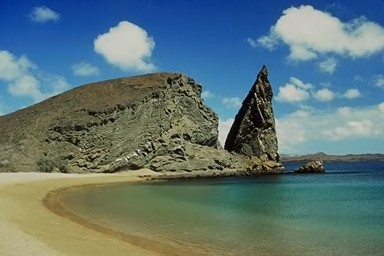
\includegraphics[width=.32\linewidth]{\detokenize{figuras/geracao/saliency-a.png}}
    }
    \subfloat[Original]{
      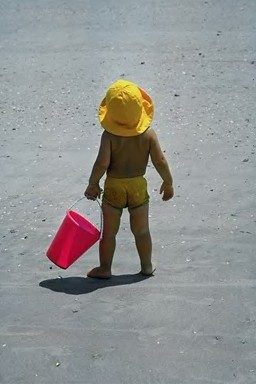
\includegraphics[width=.32\linewidth]{\detokenize{figuras/geracao/saliency-b.png}}
    }
    \subfloat[Imagem artificial]{
      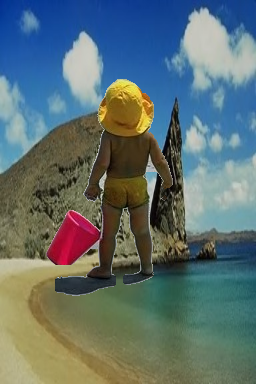
\includegraphics[width=.32\linewidth]{\detokenize{figuras/geracao/saliency-c.png}}
    }
  \end{center}
  \caption[Geração artificial utilizando a \emph{mistura saliente} de duas imagens. A imagem resultante (c) apresenta a região saliente de (b) sobreposta em (a).]{Geração artificial utilizando a \emph{mistura saliente} de duas imagens. A imagem resultante (c) apresenta a região saliente de (b) sobreposta em (a). \\ \textit{Fonte:~Elaborado pela autora.}}
  \label{fig:gen:saliency}
\end{figure}

As operações aplicadas na imagem para extrair a região mais saliente são: segmentação pelo método \sigla{SLIC}{\textit{Simple Linear Iterative Clustering}}; rotulação por conectividade; \textit{threshold} de OTSU; e operações morfológicas. O Algoritmo~\ref{alg:saliency} apresenta os passos para o cálculo do \textit{background} e \textit{foreground}.

\begin{algorithm}[!htbp]
  \caption{Geração artificial: \emph{mistura saliente}}
  \label{alg:saliency}
  \SetAlgoLined
  \Entrada{
    \begin{itemize}
      \item[] Imagem colorida $I$ em formato RGB
      \item[] Imagem colorida $I_2$ em formato RGB
    \end{itemize}
  }
  \Saida{Imagem gerada $I_{gerada}$}

  $I_{\text{rotulada por segmento}} \gets SLIC(I)$\;
  $I_{\text{mapa de saliência}} \gets \textit{rotulação por conectividade}(I_{\textit{rotulada por segmento}})$\;
  $I_{threshold} \gets OTSU(I_{\textit{mapa de saliência}})$\;
  $I_{morfologica} \gets \textit{abertura e dilatação} (I_{threshold})$\;
  $I_{foreground} \gets \textit{aplica máscara}(I_{morfologica}, I) $\;
  $I_{morfologica} \gets \textit{oposto}(I_{morfologica})$\;
  $I_{background} \gets \textit{aplica máscara}(I_{morfologica}, I_2) $\;
  $I_{gerada} \gets I_{background} + I_{foreground}$\;
\end{algorithm}

\begin{description}
  \item[Parâmetros e suas variações] Assim como no método anterior, os parâmetros são relacionados ao tamanho do elemento estruturante para a abertura e dilatação e são fixos para os experimentos desta pesquisa.

  \item[Limitações] Não é garantido que o algoritmo de saliência consiga extrair
  a melhor região, ou mesmo que sempre haja uma região saliente.

  \item[Métodos relacionados] Assemelha-se à mistura por \textit{thresholds}.
\end{description}
%%%%%%%%%%%%%%%%%%%%%%%%%%%%%%%%%%%%%%%%%%%%%%%%%%%%%%%%%%%%%%%%%%%%%%%%%%%%%%%%
\FloatBarrier
\subsection{Composição}

Essa geração pretende compor informações de diversas imagens em uma única. Assim é feito um mosaico com várias imagens, conforme pode ser visto na  Figura~\ref{fig:gen:composition}. Para cada quadrado a ser preenchido, sorteia uma imagem do conjunto de treinamento; realiza uma operação de \emph{borramento}, \emph{aguçamento}, \emph{mistura ponderada} ou \emph{SMOTE visual}; e adiciona essa imagem no quadrado respectivo. Os passos para tal \emph{composição} estão descritos no Algoritmo~\ref{alg:composition}.

\begin{figure}[!htbp]
  \begin{center}
    \centering
    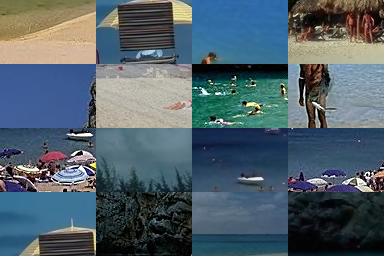
\includegraphics[width=0.6\linewidth]{\detokenize{figuras/geracao/composition.png}}
  \end{center}
  \caption[Geração artificial utilizando uma \emph{composição} de imagens. Várias imagens, dispostas em um mosaico, formam a imagem resultante. Cada célula do mosaico sofre uma operação, sorteada no momento da geração da imagem.]{Geração artificial utilizando uma \emph{composição} de imagens. Várias imagens, dispostas em um mosaico, formam a imagem resultante. Cada célula do mosaico sofre uma operação, sorteada no momento da geração da imagem. \\ \textit{Fonte:~Elaborado pela autora.}}
  \label{fig:gen:composition}
\end{figure}

\begin{algorithm}[!htbp]
  \caption{Geração artificial: \emph{composição}}
  \label{alg:composition}
  \SetAlgoLined
  \Saida{Imagem gerada $I_{gerada}$}
  \Enqto{total < \text{número de quadrados $q$}}{
  $I \gets \textit{imagem aleatória do conjunto de treinamento}$\;
  $\textit{operação} \gets \textit{número aleatório entre 1 e 4}$\;
  \Selec{\textit{operação}} {
  \uCaso{1} {
  $I \gets \emph{borramento}(I)$\;
  }
  \uCaso{2} {
  $I \gets \textit{mistura ponderada}(I)$\;
  }
  \uCaso{3} {
  $I \gets \textit{aguçamento}(I)$\;
  }
  \uCaso{4} {
  $I \gets \textit{SMOTE visual}(I)$\;
  }
  }
  $x \gets \textit{posição aleatória em x de } I$\;
  $y \gets \textit{posição aleatória em y de } I$\;
  $qx \gets \textit{posição atual para o quadrado em x de } I_{gerada}$\;
  $qy \gets \textit{posição atual para o quadrado em y de } I_{gerada}$\;
  $I_{gerada}(qx, qy) \gets I(x,y)$\;
  $total++$\;
  }
\end{algorithm}

\begin{description}
  \item[Parâmetros e suas variações] O parâmetro $q$ controla quantos quadrados são criados na imagem resultante. Nesta pesquisa, foram realizados experimentos com 4 e 16 quadrados.

  \item[Limitações] O término brusco de uma imagem para início da outra, ao formar a grade de imagens, tem efeitos colaterais de inserção de textura que, em alguns casos, não excedam a vantagem de compor uma mesma imagem com várias cores, texturas e formas das imagens originais.

  \item[Métodos relacionados] Fazer uma composição de imagens em quadrantes pode estar relacionado com a composição ao utilizar saliência.

  % \item[Visualização]
\end{description}
%%%%%%%%%%%%%%%%%%%%%%%%%%%%%%%%%%%%%%%%%%%%%%%%%%%%%%%%%%%%%%%%%%%%%%%%%%%%%%%%
% \item \underline{Redes neurais}: por representarem o estado da arte da classificação, reconhecimento e localização de objetos, as redes neurais de convolução são estudadas. Pretende-se utilizar a análise dos resultados do seu treinamento para identificar as características relevantes em imagens. Já as máquinas de Boltzmann restritas são redes neurais mais simples, portanto convenientes para a verificação da relevância de uma imagem para o aprendizado.
%  \item[Implementação:] a biblioteca \-OpenCV \cite{Intel2010} será utilizada para as funções gerais de carregar, processar, salvar e classificar imagens. A linguagem de programação para utilizar esta biblioteca e na qual esta pesquisa está sendo implementada é C++. Para a geração de gráficos das medidas estatísticas a linguagem de programação Python é utilizada. O código está disponível em \url{https://bitbucket.org/moacirponti/imagefeatureextraction/overview}.
%  \item[Bases de imagens:] considerando que os objetivos propostos possuem um viés genérico, os experimentos vão ser realizados em diversas coleções de imagens com o objetivo de estabelecer ou refutar as hipóteses levantadas.
%
%  Os resultados preliminares foram obtidos utilizando a base de imagens Corel\footnote{Disponível em http://wang.ist.psu.edu/docs/related/}, composta por fotografias que representam as classes: tribos africanas, praia, construções, ônibus, dinossauros, elefantes, flores, cavalos, montanhas e tipos de comidas. São 10 classes balanceadas com 100 imagens cada. Para fins de exemplificação, foram selecionadas imagens que representam essas classes na Figura \ref{fig:corel}.
%
%  \begin{figure}[hbpt]
%  \begin{center}
%    \includegraphics[width=1\linewidth]{\detokenize {figuras/exemplos_Corel-1000.png}}
%  \end{center}
%   \caption[Base de imagens Corel-1000.]{Base de imagens Corel-1000 utilizada. Estão representadas as 10 classes da base. \\ \textit{Fonte: Elaborado pela autora.}}
%  \label{fig:corel}
% \end{figure}
%
%
%  \item[Experimentos:] serão realizados diversos experimentos direcionados a explorar as etapas de pré-processamento, para melhorar a acurácia da classificação de bases de imagens. Como entrada são utilizadas imagens originais provenientes de diversas coleções disponíveis na literatura. Como resultado, serão calculadas medidas estatísticas da classificação dessas coleções após a alteração dessas imagens com os métodos de realce de características relevantes.
%
%  \item[Análise dos dados:] os experimentos realizados irão resultar em medidas estatísticas da classificação. A análise irá comparar a classificação das imagens originais com aquelas tratadas pelo método proposto. Ainda, o método de rebalanceamento de classes será comparado com técnicas disponíveis na literatura, como o SMOTE.
%
% \item[Forma de avaliação:]
% Por fim, a \underline{distância de Mahalanobis} também pode ser utilizada: antes e depois da geração artificial de imagens, calcular a distância entre a média das classes e a variância dentro das classes \cite{mahalanobis2000}. Ela se baseia na correlação entre as variáveis e pode ser definida por
% \begin{equation*}
%   D_m(x_i) = \sqrt{(x_i - \mu)C^{-1}(x_i-\mu)^T},
% \end{equation*}
% \noindent onde $x_i$ é um vetor de valores, $\mu$ a média e C a matriz de covariância.
%
% \end{description}
%
% %-------------------------------------------------------------------------------
% \section{Resultados esperados}
% \label{sec:resultados}
%
% Os resultados esperados são relacionados às áreas de \textbf{processamento de imagens e reconhecimento de padrões}. Espera-se obter uma comprovação das hipóteses levantadas por essa pesquisa. Os resultados são esperados em duas vertentes:
%
% \begin{enumerate}
%  \item \textit{Pré-processamento} de imagens que caracterizem melhor aspectos de suas classes, aumentando a variância entre as classes quando comparado com as imagens originais.
%  \item \textit{Geração artificial de imagens} de classes minoritárias de forma a compensar o desbalanceamento natural das bases de dados.
% \end{enumerate}
%
% Em ambos os casos pretende-se melhorar a classificação, validando-a através do cálculo da medida-F1. A análise das características aprendidas por uma rede neural de convolução será realizada ao executar o treinamento com bases específicas que destaquem propriedades como cor, textura e forma. Além disso, os resultados serão obtidos a partir da escolha de quais imagens adicionam informação ao conjunto de treino. As redes RBM serão utilizadas para este fim. Bases naturalmente não balanceadas serão testadas e seus resultados avaliados.



% \item ACC: com um conjunto de quatro distâncias $D = {1, 3, 5, 7}$ e a distância tabuleiro de xadrez $D_8(p,q) = Max(|x-s|, |y-t|)$ entre os pixels $p(x,y)$ e $q(s,t)$;
% \item \emph{BIC}: com uma vizinhança de quatro pixels;
% \item CCV: adotando um valor de $\mathit{threshold} = 25$ para a classificação dos pixels entre coerentes e incoerentes;
% \item \emph{Haralick-6}: o pixel vizinho para o qual computar a matriz de correlação foi definido como sendo o pixel à direita.

%%%%%%%%%%%%%%%%%%%%%%%%%%%%%%%%%%%%%%%%%%%%%%%%%%%%%%%%%%%%%%%%%%%%%%%%%%%%%%%%
\section{Experimentos}
\label{sec:resultados-geracao}

Esta seção descreve os resultados encontrados ao rebalancear as classes de imagens aplicando os processamentos --- descritos na seção anterior --- nas imagens originais. As imagens geradas são então utilizadas como treinamento da classe minoritária. A Figura \ref{fig:fluxo} destaca o fluxo de operações realizadas para a análise do impacto da geração de imagens no rebalanceamento de classes. O mesmo protocolo de conversão para escala de cinza, extração de características e classificação foi seguido para três sub-experimentos: base desbalanceada; base rebalanceada com interpolação dos vetores de características (método SMOTE); e base rebalanceada com a geração artificial de imagens. Alguns experimentos foram realizados com bases de imagens originalmente balanceadas. Para tais casos, foi necessário desbalancear a base para testar o rebalanceamento.

\begin{figure}[!htbp]
\centering
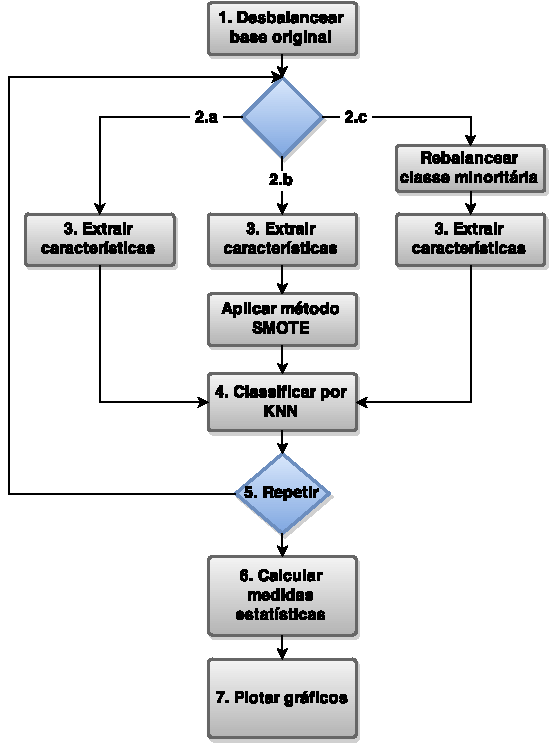
\includegraphics[scale=1.1]{\detokenize{figuras/flow_main.pdf}}
\caption[Fluxo de operações para obtenção dos resultados do rebalanceamento de classes. O mesmo protocolo de conversão para escala de cinza, extração de características e classificação foi seguido para três sub-experimentos: base desbalanceada; base rebalanceada com interpolação dos vetores de características (método SMOTE); e base rebalanceada com a geração artificial de imagens.]{Fluxo de operações para obtenção dos resultados do rebalanceamento de classes. O mesmo protocolo de conversão para escala de cinza, extração de características e classificação foi seguido para três sub-experimentos: base desbalanceada; base rebalanceada com interpolação dos vetores de características (método SMOTE); e base rebalanceada com a geração artificial de imagens. \\ \textit{Fonte:~Elaborado pela autora.}}
\label{fig:fluxo}
\end{figure}

Procurando estabilidade dos resultados obtidos com a geração das imagens artificiais, foi identificada a necessidade de controlar a remoção de imagens da base no momento da criação da base desbalanceada. Assim, os resultados foram obtidos a partir de uma forma de validação \textit{k-fold} com o objetivo de prover mais robustez ao sistema. A Figura \ref{fig:folds} ilustra como tal validação é realizada, utilizando como exemplo uma base com duas classes de imagens. Primeiramente as imagens são separadas de forma aleatória em $k = 5$ \textit{folds} em cada classe. Em seguida, as duas classes compõem 40 configurações, consistindo em todas as possibilidades de: um fold para teste e os outros como treino para a classe que permanecerá balanceada; e um de teste e apenas um de treino para a classe que os métodos de processamento irão rebalancear. Tal validação é repetida para todas as classes, ou seja, cada classe tem a possibilidade de ser a minoritária. Se originalmente a base é naturalmente desbalanceada, um \textit{fold} é utilizado para teste e os demais como treino para todas as classes.

\begin{figure}[!htbp]
\centering
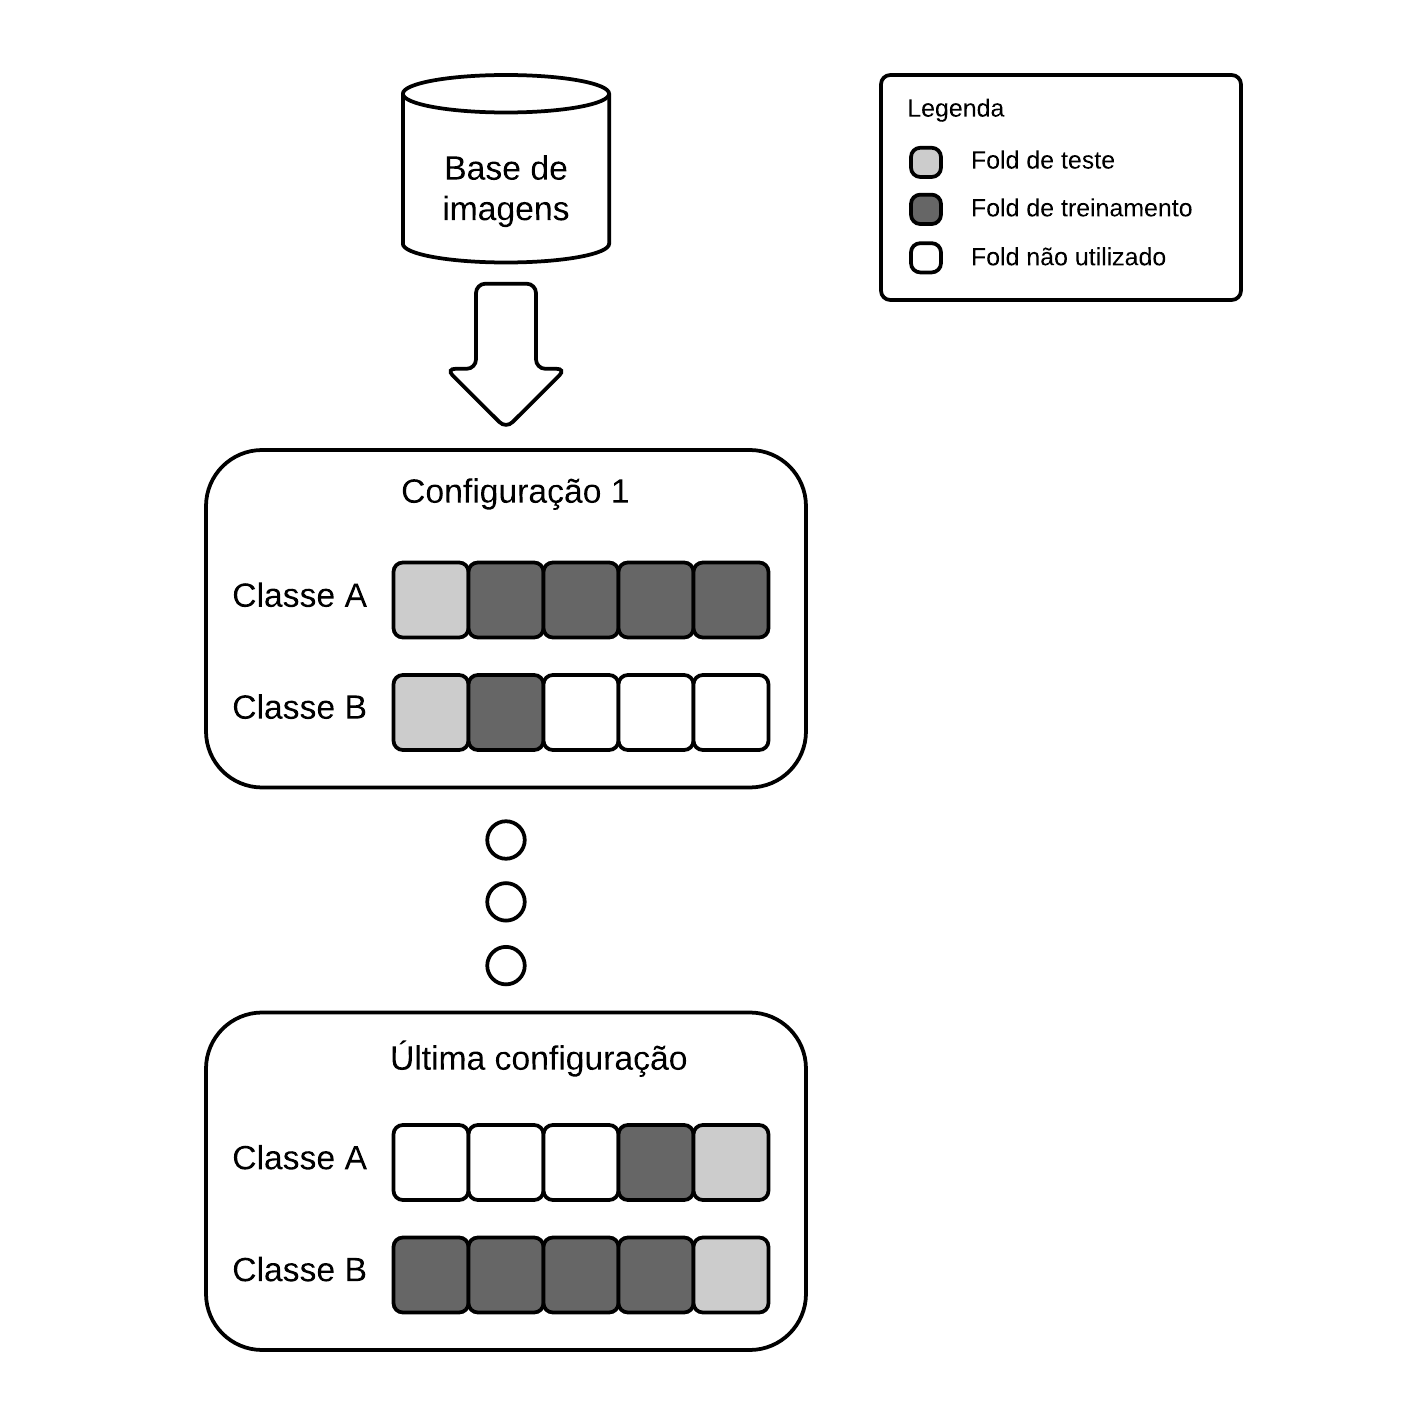
\includegraphics[scale=0.28]{\detokenize{figuras/folds_chart.png}}
\caption[Ilustração de como os experimentos de geração de imagens artificiais foram realizados. Primeiramente as imagens são separadas de forma aleatória em $k = 5$ \textit{folds} em cada classe. Em seguida, as duas classes compõem 40 configurações, consistindo em todas as possibilidades de: um fold para teste e os outros como treino para a classe que permanecerá balanceada; e um de teste e apenas um de treino para a classe que os métodos de processamento irão rebalancear. Tal validação é repetida para todas as classes, ou seja, cada classe tem a possibilidade de ser a minoritária.]{Ilustração de como os experimentos de geração de imagens artificiais foram realizados. Primeiramente as imagens são separadas de forma aleatória em $k = 5$ \textit{folds} em cada classe. Em seguida, as duas classes compõem 40 configurações, consistindo em todas as possibilidades de: um fold para teste e os outros como treino para a classe que permanecerá balanceada; e um de teste e apenas um de treino para a classe que os métodos de processamento irão rebalancear. Tal validação é repetida para todas as classes, ou seja, cada classe tem a possibilidade de ser a minoritária. \\ \textit{Fonte:~Elaborado pela autora.}}
\label{fig:folds}
\end{figure}

A acurácia pode não refletir propriamente os resultados em um cenário de bases desbalanceadas. Isso se deve ao fato de que se a classe minoritária não obtiver nenhum resultado correto e a classe majoritária tiver 100\% de acertos, tal acurária poderá ser muito alta, mesmo considerando que nenhuma imagem da classe minoritária foi corretamente classificada. Dessa forma, considera que os erros são igualmente importantes. Pode-se estender essa medida obtendo-se a acurácia balanceada: medida de acerto baseada na divisão do conjunto de objetos em teste e treinamento, realizando a repetição dos experimentos $n$ vezes e obtendo a média e o desvio padrão. A acurácia de cada experimento é obtida por

\begin{equation*}
  Acc = 1 - \frac{\sum_{i=1}^{c} E(i)}{2c},
\label{eq:Accuracy}
\end{equation*}

\noindent  que considera problemas de desbalanceamento de classes, onde $c$ é o número de classes e $E(i) = e_{i,1} + e_{i,2}$ é o erro relativo a $c$, calculado por

\begin{equation*}
  e_{i,1} = \frac{FP(i)}{N-N(i)} \,\,\,\,\, \text{ e } \,\,\,\,\, e_{i,2} = \frac{FN(i)}{N(i)}, i=1,...,c,
\label{eq:Errors}
\end{equation*}
\noindent onde $FN(i)$ são os exemplos pertencentes à classe $i$ e incorretamente classificados (falsos negativos), e $FP(i)$ são os exemplos erroneamente rotulados como~$i$ (falsos positivos). Os experimentos consideram a classe minoritária como positiva e a minoritária como negativa.

Uma outra medida, que pode efetivamente avaliar o desempenho da classificação em cenários desbalanceados, é o \textit{F1-Score}:

\begin{equation*}
  F1 = 2 \frac{PR}{P+R}.
\end{equation*}

Essa medida combina precisão e revocação como medida de efetividade da classificação \cite{Garcia2009}. A precisão é a medida da exatidão:

\begin{equation*}
  P = \frac{VP}{VP + FP},
\end{equation*}

\noindent onde $VP$ são os exemplos positivos corretamente classificados. Dos exemplos classificados como positivos, essa medida indica quantos realmente são. Ao mesmo tempo, a revocação é a medida de completude. Essa métrica indica quantos exemplos positivos foram corretamente classificados, sendo determinada por:

\begin{equation*}
  R = \frac{VP}{VP + FN}.
\end{equation*}

A partir dessas medidas estatísticas, o teste \textit{Honest Significant Difference} (HSD) de Tukey pode ser utilizado para determinar se há diferença significativa em uma amostra de resultados gerados. A hipótese nula a ser testada por estes experimentos é que não há diferença estatística relevante entre as observações de \textit{F1-Scores}. Para analisar se o teste da hipótese é significativo, pode ser utilizado o \textit{p-value}, que indica o quão estatisticamente significante o resultado é: quanto menor o seu valor, maior a evidência contra a hipótese nula (utiliza-se um limiar de 0,05).

% A partir dessas medidas, o \underline{teste estatístico de Friedman} pode ser usado para determinar se há diferença significante em uma amostra de resultados gerados \cite{friedman2010}. As performances dos algoritmos são analisados e um \textit{rank} é atribuído para cada conjunto de dados. Ele considera que a hipótese nula a ser testada é que não há diferença estatística relevante entre as observações. Para analisar se o teste da hipótese é significativo, pode ser utilizado o \underline{p-valor}, que indica o quão estatisticamente significante o resultado é: quanto menor o seu valor, maior a evidência contra a hipótese nula (geralmente o limiar utilizado é de 0,05).

A seguir, para cada experimento realizado são descritos: a base de imagens utilizada; o protocolo e parâmetros adotados; e por fim os resultados obtidos a partir de seu uso são mostrados e discutidos.

%%%%%%%%%%%%%%%%%%%%%%%%%%%%%%%%%%%%%%%%%%%%%%%%%%%%%%%%%%%%%%%%%%%%%%%%%%%%%%%%
\FloatBarrier
\subsection{Experimento 1: duas classes discriminadas}

Neste experimento foram utilizadas duas classes de fácil diferenciação, porém com alguma sobreposição. Um sub-experimento de visualização foi realizado para análise do espaço de características.
% Como o foco é na visualização de tal espaço, é relevante ter o modelo do espaço ideal das classes balanceadas. Por conta disso, esse experimento em específico não trata de uma base naturalmente desbalanceada.

%-------------------------------------------------------------------------------
\subsubsection*{Protocolo}
\begin{enumerate}
\item \textbf{Imagens originais}: classes \emph{Horse} e \emph{Elephant} da base de imagens Corel-1000, exemplificadas na Figura \ref{fig:resultados:1:base} \cite{Wang2001}. A principal característica dessas imagens é a diferença de cores, contendo pequeno grau de sobreposição.


\begin{figure}[!htbp]
  \begin{center}
    \subfloat{
      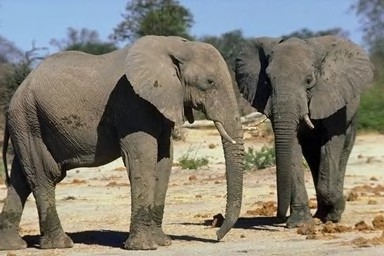
\includegraphics[width=0.48\linewidth]{\detokenize{figuras/corel_original4.jpg}}
    }
    \subfloat{
      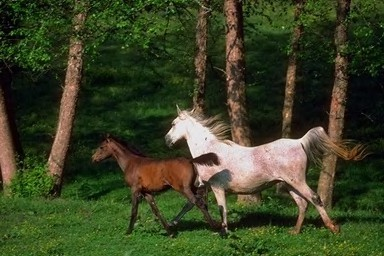
\includegraphics[width=0.48\linewidth]{\detokenize{figuras/cavalo-original2.png}}
    }

    \caption[Classes \emph{Horse} e \emph{Elephant} utilizadas no experimento. São duas classes bem discriminadas com 100 imagens cada, originalmente da base de imagens Corel-1000.]{Classes \emph{Horse} e \emph{Elephant} utilizadas no experimento. São duas classes bem discriminadas com 100 imagens cada, originalmente da base de imagens Corel-1000. \\ \textit{Fonte:~\citeonline{Hu2013}.}}
    \label{fig:resultados:1:base}
\end{center}
\end{figure}


\item \textbf{Desbalanceamento}: para o sub-experimento de visualização, cada classe foi dividida em 50\% para treino e 50\% para teste, de maneira aleatória. Após, a classe \emph{Horse} sofreu remoção de 88\% do seu conjunto de treino, tornando-a desbalanceada. Já para a análise estatística do experimento, todas as 40 configurações de \textit{folds} com $k=5$ foram realizadas (padronização anteriormente descrita na Figura~\ref{fig:folds}).

\item \textbf{Método para geração artificial}: para a visualização do espaço de características foi utilizado o método de \emph{mistura} de duas imagens originais, exemplificado na Figura~\ref{fig:mistura}. Para a análise do \textit{boxplot} de \textit{F1-Scores}, todas as gerações foram testadas e os resultados são reportados a seguir.


\begin{figure}[!htbp]
  \begin{center}
    \subfloat[Original]{
      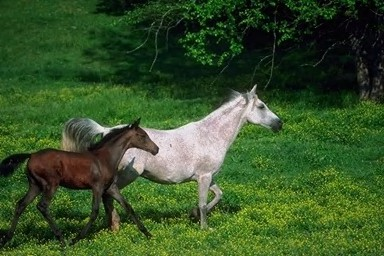
\includegraphics[width=.32\linewidth]{\detokenize{figuras/cavalo-original.png}}
    }
    \subfloat[Original]{
      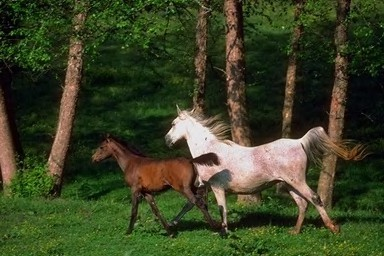
\includegraphics[width=.32\linewidth]{\detokenize{figuras/cavalo-original2.png}}
    }
    \subfloat[Imagem artificial]{
      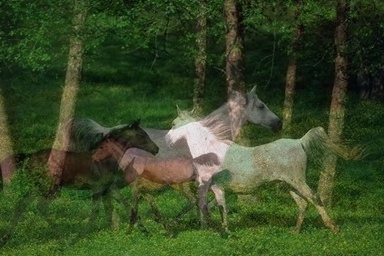
\includegraphics[width=.32\linewidth]{\detokenize{figuras/cavalo-blend.png}}
    }
    \caption[Exemplo da geração artificial de imagens com o método de \emph{mistura} para as classes \emph{Elephant} e \emph{Horse} da base Corel-1000. A imagem resultante (c) é composta pela mistura de (a) e (b).]{Exemplo da geração artificial de imagens com o método de \emph{mistura} para as classes \emph{Elephant} e \emph{Horse} da base Corel-1000. A imagem resultante (c) é composta pela mistura de (a) e (b). \\ \textit{Fonte:~Elaborado pela autora.}}
    \label{fig:mistura}
\end{center}
\end{figure}


\item \textbf{Conversão em escala de cinza}: método \emph{Intensidade'} para a visualização. Todas as combinações de extração e conversão em escala de cinza foram testadas, portanto todos os métodos de conversão foram utilizados.

\item \textbf{Extração de características}: classificação de pixels de borda e interior (BIC) para a visualização. Todos os métodos de extração foram testados para a análise estatística.

\item \textbf{Classificação}: o classificador supervisionado KNN com $K=1$ (para mais detalhes ver Seção~\ref{sec:knn}) foi utilizado.

\item \textbf{Projeção multidimensional para visualização}: dois componentes principais encontrados ao aplicar PCA (Seção~\ref{sec:pca}) nos vetores de características para redução de dimensionalidade foram projetados.
\end{enumerate}

%-------------------------------------------------------------------------------
\subsubsection*{Visualização}

A visualização do espaço de características obtido após a geração artificial de imagens pode ajudar a verificar se as novas imagens melhoram a definição da classe minoritária em relação ao espaço original. Ou seja, se o método utilizado revelou características latentes. Dessa forma, ao projetar os novos vetores no espaço das imagens originais, é possível analisar qual método --- SMOTE ou geração de imagens no campo visual --- mais se assemelha à distribuição original dos dados.

As classes \emph{Elephant} e \emph{Horse} possuem 100 imagens cada. O primeiro passo foi remover imagens de uma das classes, tornando a base desbalanceada. Na Figura~\ref{fig:desbalanceado} está ilustrada a remoção de 88\% das imagens de treino da classe \emph{Horse}, originalmente balanceada. Essa e as próximas projeções desta seção foram obtidas com a técnica para redução de dimensionalidade PCA, descrita na Seção~\ref{sec:pca}, e são referentes aos dois componentes principais com maiores autovalores.

\begin{figure}[!htbp]
  \begin{center}
    \subfloat[Original]{
      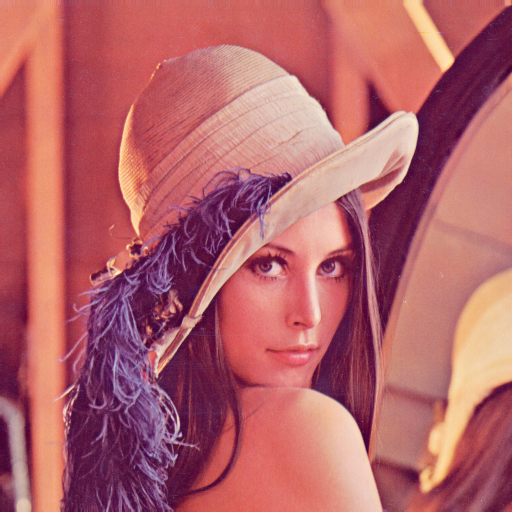
\includegraphics[width=.48\linewidth]{\detokenize{figuras/visualizacao/original.png}}
    }
    \subfloat[Desbalanceado]{
      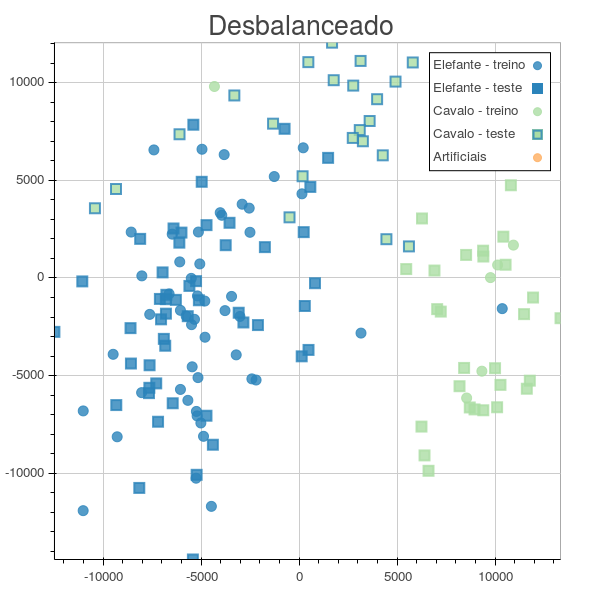
\includegraphics[width=.48\linewidth]{\detokenize{figuras/visualizacao/desbalanceado-fixed.png}}
    }
\end{center}
\caption[À esquerda a projeção dos dois componentes principais obtidos com a aplicação de PCA nas classes \emph{Elephant} --- em azul --- e \emph{Horse} --- em verde. À direita, as mesmas classes após a remoção de 88\% das imagens de treino da classe \emph{Horse}. A diferença dos marcadores consiste na definição de imagens para treino e teste não existente nas classes originais.]{À esquerda a projeção dos dois componentes principais obtidos com a aplicação de PCA nas classes \emph{Elephant} --- em azul --- e \emph{Horse} --- em verde. À direita, as mesmas classes após a remoção de 88\% das imagens de treino da classe \emph{Horse}. A diferença dos marcadores consiste na definição de imagens para treino e teste não existente nas classes originais. \\ \textit{Fonte:~Elaborado pela autora.}}
\label{fig:desbalanceado}
\end{figure}

Os resultados da classificação dos três experimentos (desbalanceado, SMOTE e geração artificial) utilizando K-NN com $K=1$ reportou que o \textit{F1-Score} da geração de imagens utilizando o método de \emph{mistura} obteve um ganho de mais de 10\% em relação ao rebalanceamento no espaço de características com o SMOTE. Foi utilizado BIC como método de extração de características e \emph{Intensidade'} como método de conversão em escala de cinza. Para essa combinação, a geração de imagens utilizando \emph{mistura} se mostrou favorável e portanto a visualização do espaço de características apresenta esse método como geração.

% \begin{figure}[!htbp]
%   \begin{center}
%       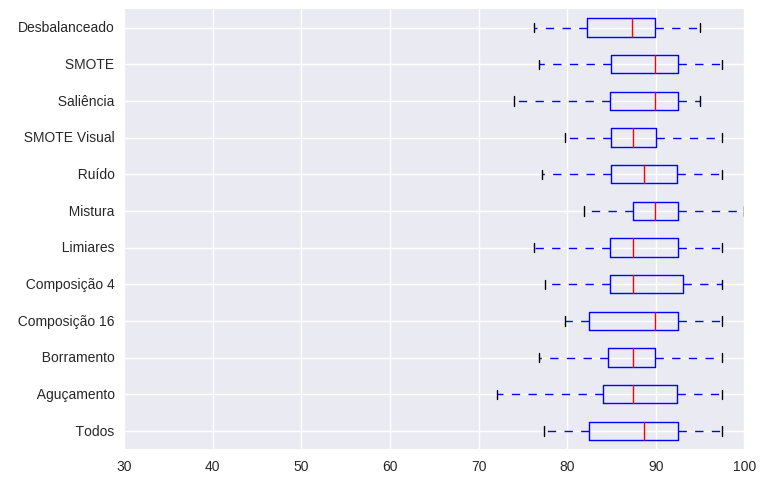
\includegraphics[width=\linewidth]{\detokenize{figuras/resultados/1/BIC_Intensity_elefante-cavalo.png}}
%     \caption[Resultados de \textit{F1-Score} para as classes \emph{Horse} e \emph{Elephant} da base Corel-1000. Foi utilizado \emph{BIC} como método de extração de características e \emph{Intensidade'} como método de conversão em escala de cinza. Para essa combinação, a geração de imagens utilizando \emph{mistura} se mostrou favorável.]{Resultados de \textit{F1-Score} para as classes \emph{Horse} e \emph{Elephant} da base Corel-1000. Foi utilizado \emph{BIC} como método de extração de características e \emph{Intensidade'} como método de conversão em escala de cinza. Para essa combinação, a geração de imagens utilizando \emph{mistura} se mostrou favorável. \\ \textit{Fonte:~Elaborado pela autora.}}
%     \label{fig:resultados:1:vis}
% \end{center}
% \end{figure}

% \begin{table}[!htbp]
% \centering
% \caption{Resultados de \textit{F1-Score} para as classes \emph{Horse} e \emph{Elephant}, utilizando \emph{Intensidade'} como método para conversão em escala de cinza e \emph{BIC} para extração de características.}
% \label{fig:resultados:1:tabvis}
% \begin{tabular}{|l|c|c|}
% \hline
% \textbf{Intensidade' e BIC} & \textbf{Média} & \textbf{Desvio padrão} \\ \hline
% Todos                      & 88.07          & 5.30                   \\ \hline
% Aguçamento                 & 86.65          & 7.00                   \\ \hline
% Borramento                 & 87.17          & 5.10                   \\ \hline
% Composição 16              & 88.16          & 5.32                   \\ \hline
% Composição 4               & 88.12          & 5.45                   \\ \hline
% Limiares                   & 87.65          & 5.10                   \\ \hline
% Mistura                    & \textbf{88.84} & 5.03          \\ \hline
% Ruído                      & 87.95          & 5.75                   \\ \hline
% SMOTE Visual               & 87.69          & 5.28                   \\ \hline
% Saliência                  & 88.09          & 5.58                   \\ \hline
% SMOTE                      & 88.55          & 5.21                   \\ \hline
% Desbalanceado              & 85.82          & 5.69                   \\ \hline
% \end{tabular}
% \end{table}

Para verificar se a geração de imagens inseriu mais informação na classe minoritária do que apenas povoar os espaços entre os exemplos, a classe rebalanceada utilizando ambos métodos está demonstrada na Figura~\ref{fig:compara_vis_treino_fixed}. Em laranja estão representados os novos exemplos de treinamento, projetados no plano da base original balanceada.

\begin{figure}[!htbp]
  \begin{center}
    \subfloat[SMOTE]{
      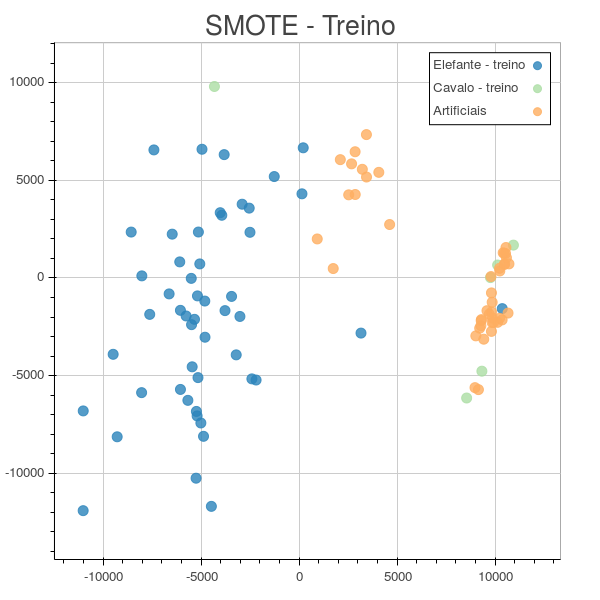
\includegraphics[width=.5\linewidth]{\detokenize{figuras/visualizacao/smote-treino-fixed.png}}
    }
    \subfloat[Geração artificial de imagens]{
      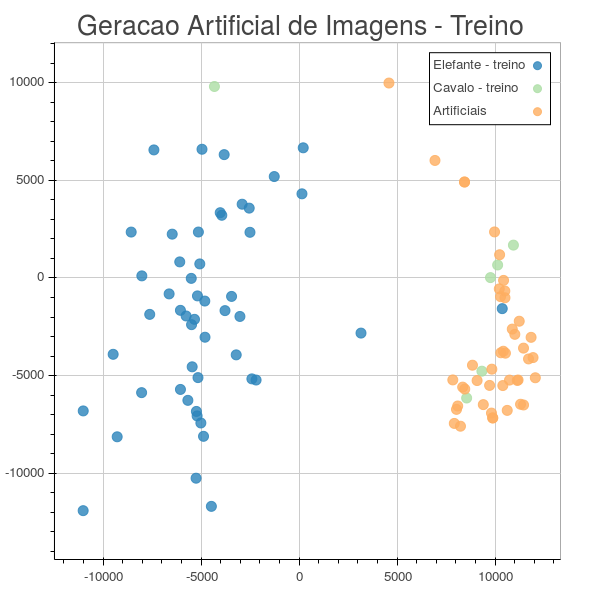
\includegraphics[width=.5\linewidth]{\detokenize{figuras/visualizacao/geracao-treino-fixed.png}}
    }
  \end{center}
  \caption[Comparação dos exemplos de treinamento da geração com SMOTE e no campo visual. Em laranja estão representados os novos exemplos, projetados no plano da base original balanceada.]{Comparação dos exemplos de treinamento da geração com SMOTE e no campo visual. Em laranja estão representados os novos exemplos, projetados no plano da base original balanceada. \\ \textit{Fonte:~Elaborado pela autora.}}
  \label{fig:compara_vis_treino_fixed}
\end{figure}

Após o treinamento realizado com as novas imagens geradas e as originais, o conjunto de teste foi fornecido ao classificador K-NN com $K = 1$ e o resultado das predições está ilustrado na Figura~\ref{fig:compara_vis_teste}. A cor no interior dos marcadores quadrados representa a classe real dos exemplos e a borda representa a classe predita pelo classificador. Nota-se que a melhoria na classificação com a geração de imagens fica visível e corresponde ao aumento do \textit{F1-Score}.

\begin{figure}[!htbp]
  \begin{center}
    \subfloat[Smote]{
      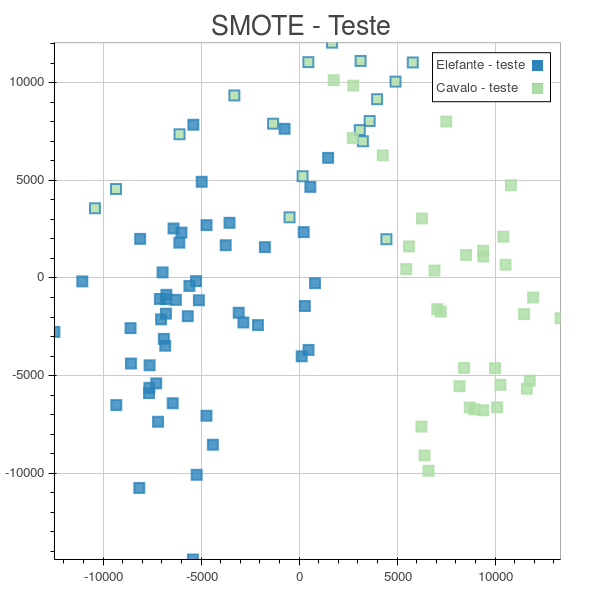
\includegraphics[width=.5\linewidth]{\detokenize{figuras/visualizacao/smote-teste-fixed.png}}
    }
    \subfloat[Geração artificial]{
      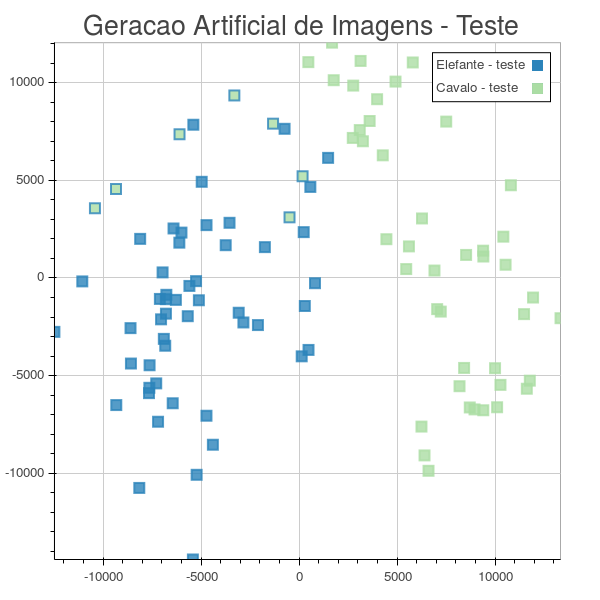
\includegraphics[width=.5\linewidth]{\detokenize{figuras/visualizacao/geracao-teste-fixed.png}}
    }
\end{center}
\caption[Resultado do teste da classificação com K-NN com $K = 1$ após o treinamento realizado com as bases rebalanceadas. A cor no interior dos marcadores quadrados representa a classe real dos exemplos e a borda representa a classe predita pelo classificador.]{Resultado do teste da classificação com K-NN com $K = 1$ após o treinamento realizado com as bases rebalanceadas. A cor no interior dos marcadores quadrados representa a classe real dos exemplos e a borda representa a classe predita pelo classificador. \\ \textit{Fonte:~Elaborado pela autora.}}
\label{fig:compara_vis_teste}
\end{figure}

De uma forma geral, pode-se dizer que a geração de imagens melhorou a definição da classe minoritária e foi o método que mais se assemelhou à distribuição dos dados originais. Além disso, um dos problemas do SMOTE pode ser verificado nessas projeções: \textbf{ao realizar a interpolação dos vetores de características originais, exemplos podem ser criados em regiões do espaço que fazem parte da outra classe}. Ficou claro também que o método SMOTE não apresentou capacidade de extrapolar a sua região, como pode ser observado no grupo de exemplos à direita do espaço de características. O SMOTE gerou novos elementos próximos a uma linha reta, enquanto a geração de imagens proporcionou uma abrangência maior em volta desse espaço, com maior dispersão.

Na Figura \ref{fig:region} é possível visualizar a região de decisão, observando suas modificações frente aos métodos. Pode ser observado que, em ambas as técnicas, a região da classe minoritária apresenta-se melhor representada. Além disso, é possível verificar que o SMOTE ocasionou uma certa invasão do espaço de características da classe majoritária.

\begin{figure}[!htbp]
    \begin{center}
    \subfloat[Desbalanceado]{
      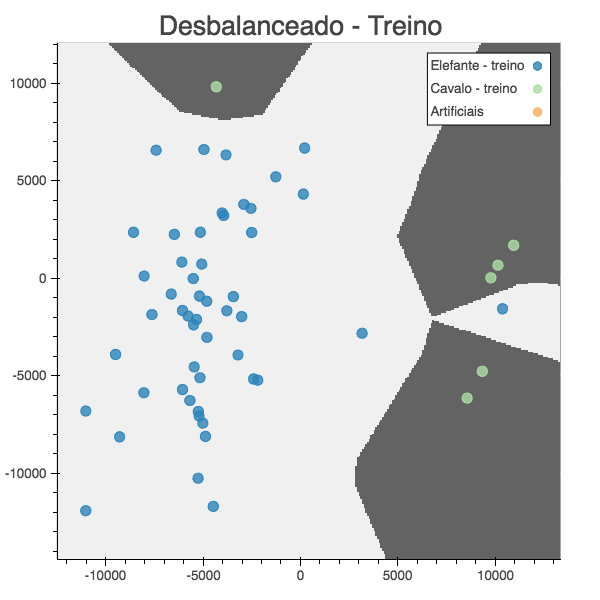
\includegraphics[width=.5\linewidth]{\detokenize{figuras/visualizacao/desbalanceado-treino-region.png}}
    }
    \end{center}
    \subfloat[Smote]{
      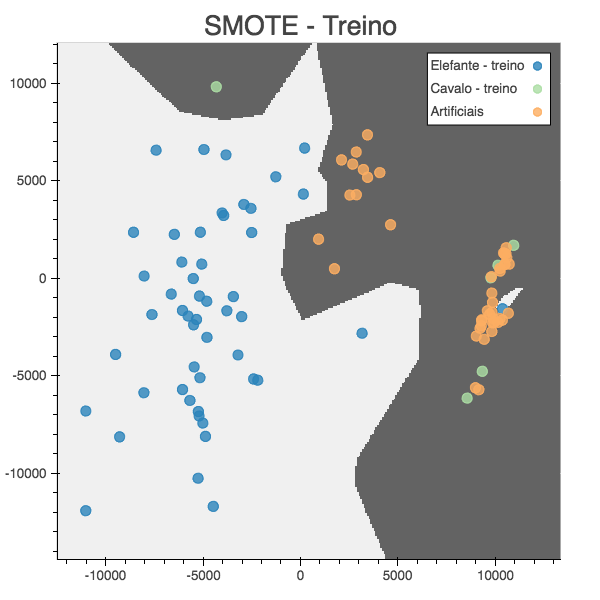
\includegraphics[width=.5\linewidth]{\detokenize{figuras/visualizacao/smote-treino-region.png}}
    }
    \subfloat[Geração artificial]{
      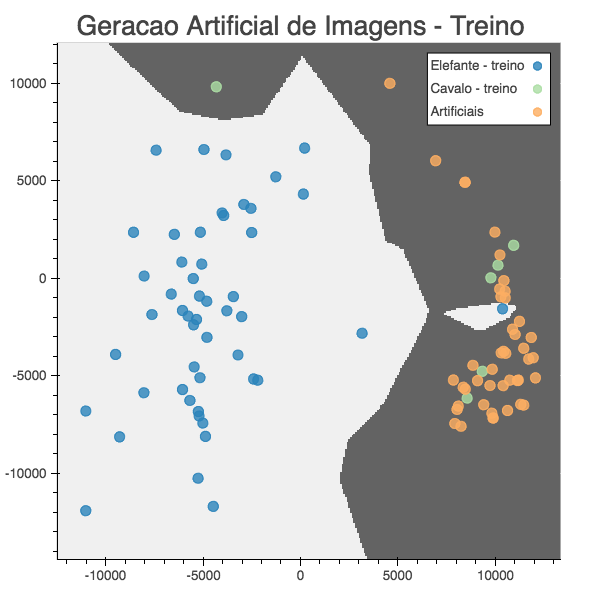
\includegraphics[width=.5\linewidth]{\detokenize{figuras/visualizacao/geracao-treino-region.png}}
    }
  \caption[Região de decisão com K-NN (K = 1). Pode ser observado que em ambas as técnicas a região da classe minoritária apresenta-se melhor representada. Além disso, é possível verificar que o SMOTE ocasionou uma certa invasão do espaço de características da classe majoritária.]{Região de decisão com K-NN (K = 1). Pode ser observado que em ambas as técnicas a região da classe minoritária apresenta-se melhor representada. Além disso, é possível verificar que o SMOTE ocasionou uma certa invasão do espaço de características da classe majoritária. \\ \textit{Fonte:~Elaborado pela autora.}}
  \label{fig:region}
\end{figure}

Em todas as figuras anteriores relacionadas a essa visualização, os exemplos foram projetados no plano criado pelas suas componentes principais com maior autovalores da base original balanceada. Se após a geração de novos exemplos essas componentes forem recalculadas (Figura \ref{fig:compara_vis_treino}), pode-se notar que a geração de imagens artificiais proporciona a criação de um subespaço que melhor discretiza as classes, quando comparado com SMOTE ou com a base desbalanceada.

\begin{figure}[!htbp]
    \begin{center}
    \subfloat[Desbalanceado]{
      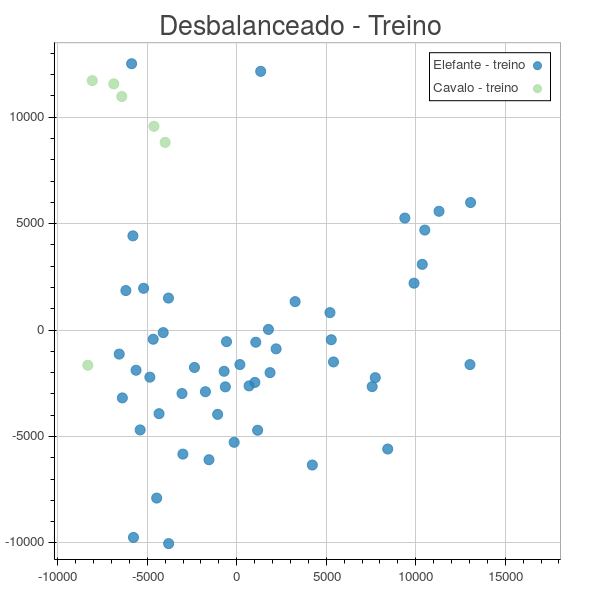
\includegraphics[width=.5\linewidth]{\detokenize{figuras/visualizacao/desbalanceado-treino.png}}
    }
    \end{center}
    \subfloat[Smote]{
      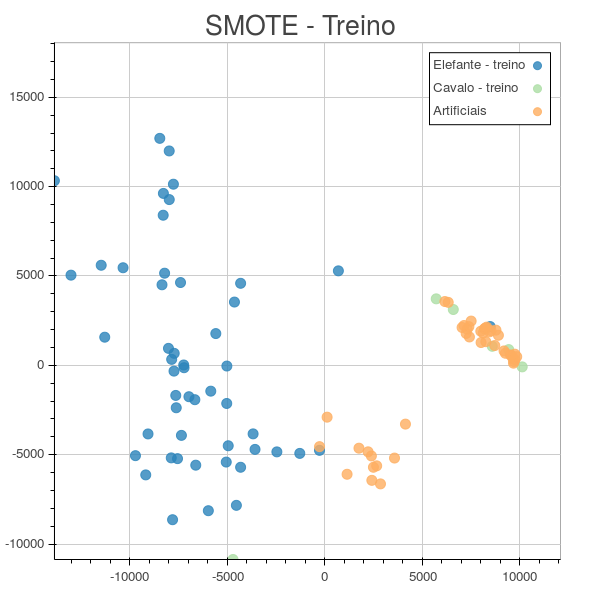
\includegraphics[width=.5\linewidth]{\detokenize{figuras/visualizacao/smote-treino.png}}
    }
    \subfloat[Geração artificial]{
      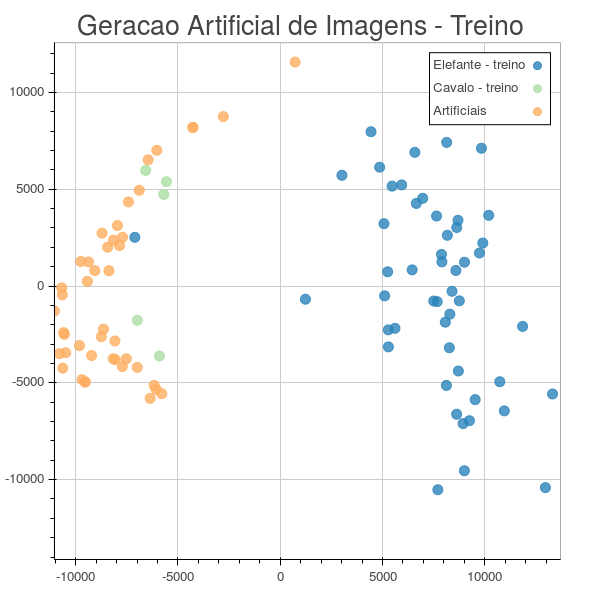
\includegraphics[width=.5\linewidth]{\detokenize{figuras/visualizacao/geracao-treino.png}}
    }
  \caption[Melhores subespaços encontrados após a geração de novos exemplos para o SMOTE, para a geração artificial de imagens, e após a remoção de imagens para a projeção dos dados desbalanceados. Pode-se notar que a geração de imagens artificiais proporciona a criação de um subespaço que melhor discretiza as classes, quando comparado com SMOTE ou com a base desbalanceada.]{Melhores subespaços encontrados após a geração de novos exemplos para o SMOTE, para a geração artificial de imagens, e após a remoção de imagens para a projeção dos dados desbalanceados. Pode-se notar que a geração de imagens artificiais proporciona a criação de um subespaço que melhor discretiza as classes, quando comparado com SMOTE ou com a base desbalanceada. \\ \textit{Fonte:~Elaborado pela autora.}}
  \label{fig:compara_vis_treino}
\end{figure}

Como relatado no início desse experimento, o extrator de características utilizado foi o BIC. Fundamentalmente ele captura informações de intensidade de cor das imagens. Na Figura~\ref{fig:vis_images} as próprias imagens foram utilizadas como marcadores na projeção do melhor subespaço após a geração artificial com o método de \emph{mistura}. É nítido o impacto da etapa de extração de características na separação das classes e também no método de geração de imagens antes de tal extração.

\begin{figure}[!htbp]
    \begin{center}
      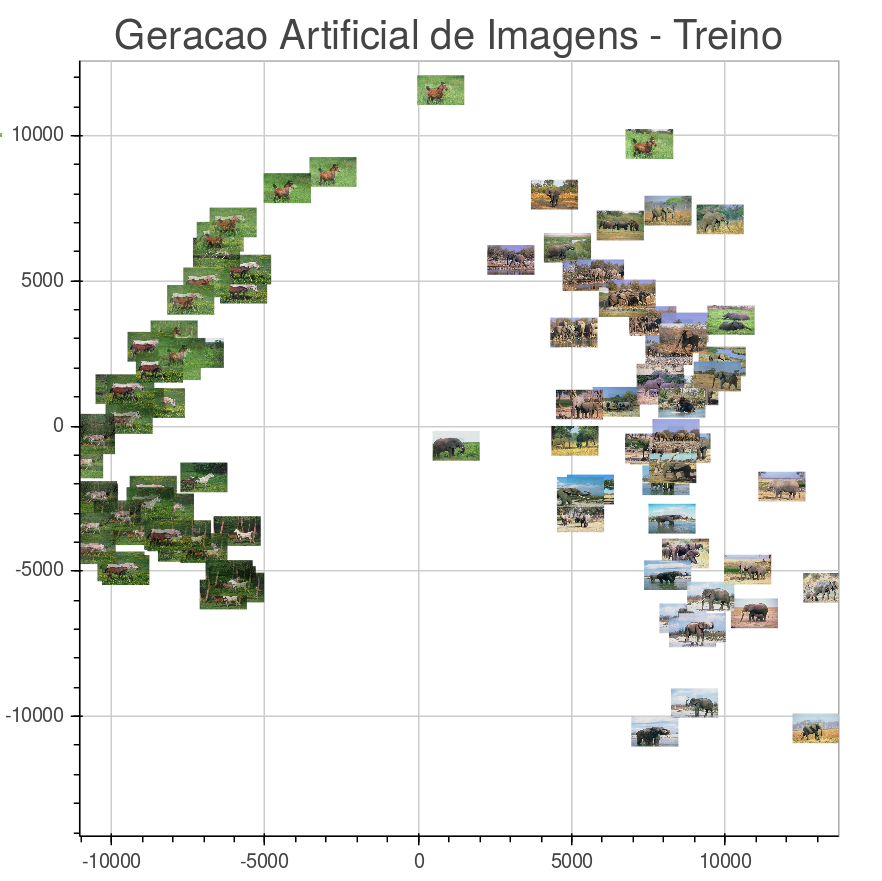
\includegraphics[width=.8\linewidth]{\detokenize{figuras/visualizacao/vis-images.png}}
    \end{center}
  \caption[Visualização do impacto do método de extração de características na separação entre classes. Possível verificar que o BIC utiliza as intensidades como principal representação de uma imagem.]{Visualização do impacto do método de extração de características na separação entre classes. Possível verificar que o BIC utiliza as intensidades como principal representação de uma imagem. \\ \textit{Fonte:~Elaborado pela autora.}}
  \label{fig:vis_images}
\end{figure}

%-------------------------------------------------------------------------------
\subsubsection*{Resultados}

Para análise estatística, todas as combinações de conversão para escala de cinza e métodos de extração de características foram testados. A combinação \emph{Gleam} e ACC obteve o melhor \textit{F1-Score} para as classes \emph{Elephant} e \emph{Horse}. O \textit{boxplot} apresentado na Figura \ref{fig:resultados:1:melhor} retrata a média dos \textit{F1-Scores} das 40 combinações deste experimento. A Tabela \ref{fig:resultados:1:tabmelhor} mostra os valores de tal métrica para o cálculo dos testes estatísticos. O método de \textit{composição}, exemplificado na Figura \ref{fig:resultados:1:composicao}, obteve o melhor \textit{F1-Score} para esse cenário.

\begin{figure}[!htbp]
  \begin{center}
      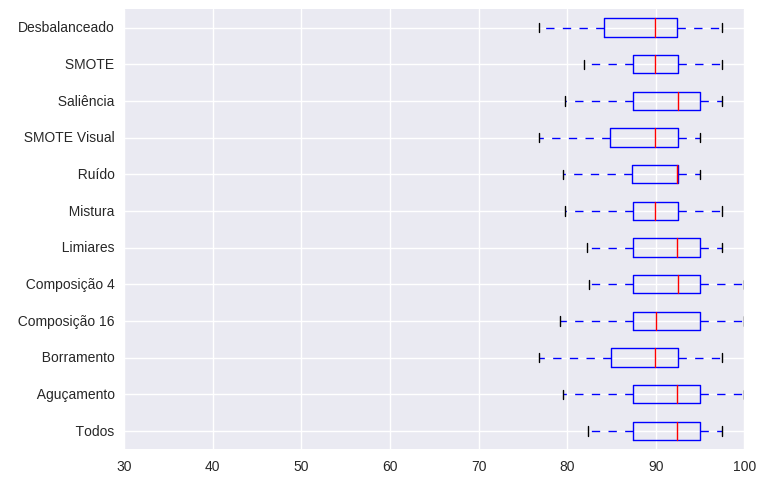
\includegraphics[width=\linewidth]{\detokenize{figuras/resultados/1/ACC_Gleam_elefante-cavalo.png}}
  \end{center}
  \caption[Conversão em escala de cinza com \emph{Gleam} e ACC como método de extração de características. Nota-se que o método de geração baseado em Composição 4 obteve maior valor de \textit{F1-Score}.]{Conversão em escala de cinza com \emph{Gleam} e ACC como método de extração de características. Nota-se que o método de geração baseado em Composição 4 obteve maior valor de \textit{F1-Score}. \\ \textit{Fonte:~Elaborado pela autora.}}
  \label{fig:resultados:1:melhor}
\end{figure}

\begin{table}[!htbp]
\begin{center}
\caption{Resultados de \textit{F1-Score} para as classes \emph{Horse} e \emph{Elephant}, utilizando \emph{Gleam} como método para conversão em escala de cinza e ACC para extração de características. Nota-se que o método de geração baseado em Composição 4 obteve maior valor de \textit{F1-Score}.}
\label{fig:resultados:1:tabmelhor}
\begin{tabular}{|l|c|c|}
\hline
\textbf{\emph{Gleam} \& ACC} & \textbf{Média}     & \textbf{Desvio Padrão} \\ \hline
Todos                 & 91.090913          & 4.559066               \\ \hline
Aguçamento            & 91.002678          & 4.907016               \\ \hline
Borramento            & 89.394500          & 5.103498               \\ \hline
Composição 16         & 90.934305          & 4.399334               \\ \hline
Composição 4          & \textbf{91.773528} & 4.909852               \\ \hline
Limiares              & 90.893133          & 5.285833               \\ \hline
Mistura               & 90.177055          & 4.409787               \\ \hline
Ruído                 & 89.337770          & 5.169757               \\ \hline
SMOTE Visual          & 88.616535          & 5.567976               \\ \hline
Saliência             & 91.282655          & 4.230281               \\ \hline
SMOTE                 & 90.173808          & 4.566863               \\ \hline
Desbalanceado         & 88.258567          & 5.538461               \\ \hline
\end{tabular}
\end{center}
\end{table}

\begin{figure}[!htbp]
  \begin{center}
    \subfloat[Imagem gerada]{
      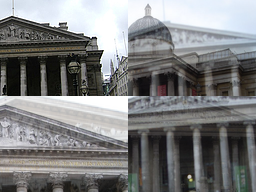
\includegraphics[width=.6\linewidth]{\detokenize{figuras/resultados/1/resultado-composicao.png}}
    }
  \end{center}
\caption[A imagem gerada apresenta uma \emph{composição} de quatro imagens da classe \textit{Elephant}.]{A imagem gerada apresenta uma \emph{composição} de quatro imagens da classe \textit{Elephant}. \\ \textit{Fonte:~Elaborado pela autora.}}
\label{fig:resultados:1:composicao}
\end{figure}

Considerando a análise da melhor combinação dos métodos de representação da imagem, foi verificado também o desempenho dos rebalanceamentos em um cenário mais complexo: o de maior variância dos \textit{F1-Scores}, dadas as 40 combinações da validação. A Figura~\ref{fig:resultados:1:pior} mostra o gráfico de \textit{boxplot} referente aos resultados da Tabela~\ref{fig:resultados:1:tabpior}. O melhor método de rebalanceamento para tal cenário foi o de geração artificial de imagens de \textit{adição de ruído}, exemplificado na Figura~\ref{fig:resultados:1:ruido}. O par de métodos MSB e HOG obteve maior valor de variância --- para conversão de escala de cinza e extração de características, respectivamente.

\begin{figure}[!htbp]
    \begin{center}
      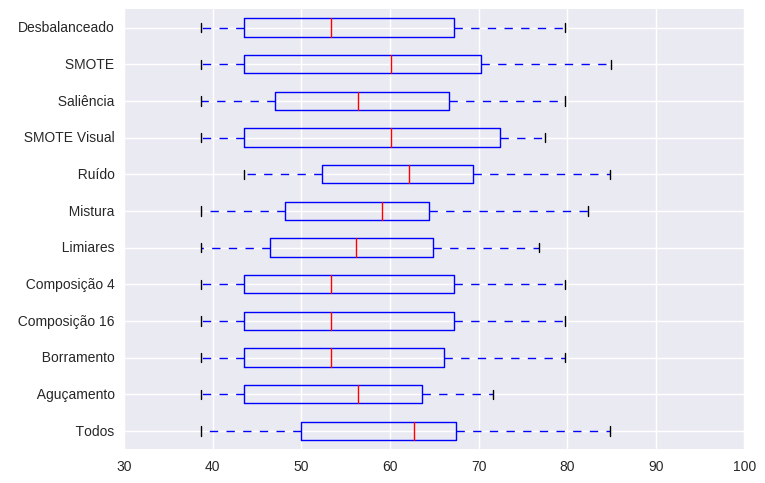
\includegraphics[width=\linewidth]{\detokenize{figuras/resultados/1/HOG_MSB_elefante-cavalo.png}}
    \end{center}
    \caption[Conversão em escala de cinza com MSB e HOG como método de extração de características. Essa combinação de métodos obteve a maior variância de \textit{F1-Score}. Nota-se que o método de \textit{adição de ruído} apresentou-se como o melhor.]{Conversão em escala de cinza com MSB e HOG como método de extração de características. Essa combinação de métodos obteve a maior variância de \textit{F1-Score}. Nota-se que a \textit{adição de ruído} apresentou-se como o melhor método. \\ \textit{Fonte:~Elaborado pela autora.}}
    \label{fig:resultados:1:pior}
\end{figure}

\begin{table}[!htbp]
\begin{center}
\caption{Resultados de \textit{F1-Score} para as classes \emph{Horse} e \emph{Elephant}, utilizando MSB como método para conversão em escala de cinza e HOG para extração de características. O método de \emph{adição de ruído} foi aquele que obteve melhor valor de \textit{F1-Score}.}
\label{fig:resultados:1:tabpior}
\begin{tabular}{|l|c|c|}
\hline
\textbf{MSB \& HOG} & \textbf{Média}     & \textbf{Desvio Padrão} \\ \hline
Todos               & 60.000127          & 12.063967              \\ \hline
Aguçamento          & 54.809555          & 10.610213              \\ \hline
Borramento          & 55.588173          & 13.275734              \\ \hline
Composição 16       & 55.667145          & 13.341421              \\ \hline
Composição 4        & 55.652205          & 13.323408              \\ \hline
Limiares            & 55.652268          & 11.547820              \\ \hline
Mistura             & 57.826535          & 10.882912              \\ \hline
Ruído               & \textbf{62.174910} & 10.746760              \\ \hline
SMOTE Visual        & 58.920085          & 14.765860              \\ \hline
Saliência           & 56.322367          & 12.169296              \\ \hline
SMOTE               & 58.342450          & 13.768688              \\ \hline
Desbalanceado       & 55.667145          & 13.341421              \\ \hline
\end{tabular}
\end{center}
\end{table}

\begin{figure}[!htbp]
  \begin{center}
    \subfloat[Original]{
      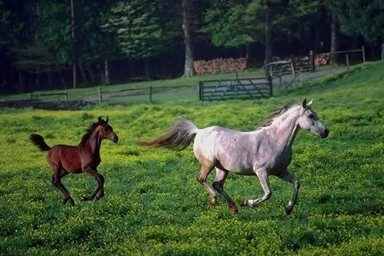
\includegraphics[width=.48\linewidth]{\detokenize{figuras/resultados/1/original-ruido.png}}
    }
    \subfloat[Imagem gerada]{
      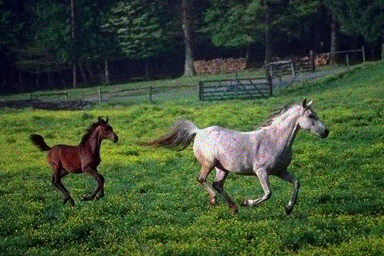
\includegraphics[width=.48\linewidth]{\detokenize{figuras/resultados/1/resultado-ruido.png}}
    }
 \end{center}
 \caption[Imagem gerada utilizando \emph{adição de ruído} em imagens da classe \emph{Horse}. Regiões mais escuras apresentam maior ruído na imagem resultante (b).]{Imagem gerada utilizando \emph{adição de ruído} em imagens da classe \emph{Horse}. Regiões mais claras apresentam maior ruído na imagem resultante (b).\\ \textit{Fonte:~Elaborado pela autora.}}
 \label{fig:resultados:1:ruido}
\end{figure}

%-------------------------------------------------------------------------------
% \FloatBarrier
\subsubsection*{Discussão}

% Tukey HSD Post-hoc Test...
% Group 1 vs Group 2: Diff=1.9152, 95%CI=-0.7500 to 4.5805, p=0.2073
% Group 1 vs Group 3: Diff=3.5150, 95%CI=0.8497 to 6.1802, p=0.0062
% Group 2 vs Group 3: Diff=1.5997, 95%CI=-1.0656 to 4.2650, p=0.3315

Interessante notar que, ao menos para este caso, a preferência pelo método de geração parece estar relacionada ao método de extração. Isso se deve, possivelmente, ao fato de o melhor método de extração indicar as características mais relevantes das imagens. Nesse caso, para as classes \emph{Elephant} e \emph{Horse} nas quais as características de cor parecem ser as mais relevantes, o melhor método de geração foi o de compôr um mosaico de diversas imagens combinado com o método de extração ACC, que captura a correlação espacial entre pixels com a mesma intensidade.

Para o resultado da combinação dos melhores métodos de conversão em escala de cinza e extração de características, o teste \textit{post-hoc} HSD de Tukey revelou que não há diferença estatística entre a base desbalanceada e o SMOTE ($\textit{p-value} = 0.2073$). Mas indicou que existe uma significância entre a base desbalanceada e ela rebalanceada com a geração de imagens artificiais ($\textit{p-value} = 0.0062$). Isso significa que o melhor método para rebalancear essas classes é a geração artificial utilizando o método de \emph{composição} de quatro imagens. Ainda de acordo com o teste, não há evidência estatística da relevância do resultado da combinação de maior variância. Portanto, todos os próximos experimentos relatam apenas os resultados da melhor combinação.

%%%%%%%%%%%%%%%%%%%%%%%%%%%%%%%%%%%%%%%%%%%%%%%%%%%%%%%%%%%%%%%%%%%%%%%%%%%%%%%%
\subsection{Experimento 2: duas classes sobrepostas}

O experimento anterior considerou classes relativamente distintas. Por isso, classes de difícil diferenciação também foram testadas e são reportadas a seguir, com o objetivo de verificar o desempenho do método.

\subsubsection*{Protocolo}
\begin{enumerate}
\item \textbf{Imagens originais}: as classes \textit{Beach} e \textit{Mountain} foram escolhidas por serem as classes que possuem maior dificuldade de diferenciação da base Corel-1000~\cite{Wang2001}. Apresentam alta taxa de sobreposição de intensidades de cores e texturas, conforme testes realizados. Uma imagem de exemplo de cada classe é apresentada na Figura~\ref{fig:resultados:2:base}.

\begin{figure}[!htbp]
  \begin{center}
    \subfloat[Mountain]{
      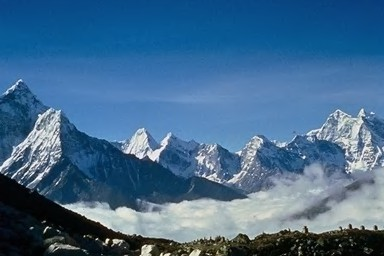
\includegraphics[width=.48\linewidth]{\detokenize{figuras/resultados/2/montanha.png}}
    }
    \subfloat[Beach]{
      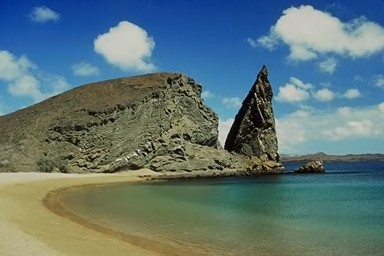
\includegraphics[width=.48\linewidth]{\detokenize{figuras/resultados/2/praia.png}}
    }
\end{center}
\caption[Imagens representativas das classes \textit{Beach} e \textit{Mountain} da base de imagens Corel-1000. Tais classes apresentam sobreposição de características por ambas apresentarem paisagens naturais. O objetivo desse experimento é verificar o desempenho da geração artificial em um problema de difícil classificação.]{Imagens representativas das classes \textit{Beach} e \textit{Mountain} da base de imagens Corel-1000. Tais classes apresentam sobreposição de características por ambas apresentarem paisagens naturais. O objetivo desse experimento é verificar o desempenho da geração artificial em um problema de difícil classificação. \\ \textit{Fonte:~\citeonline{Wang2001}.}}
\label{fig:resultados:2:base}
\end{figure}

\item \textbf{Desbalanceamento}: as duas classes contém 100 imagens cada, portanto são balanceadas. Para esse experimento, foram utilizadas as 40 combinações de desbalanceamento dos $k=5$ folds.

\item \textbf{Método para geração artificial}: todos os métodos de geração foram testados. Os que obtiveram melhores resultados foram os métodos de: \textit{mistura saliente}, \emph{aguçamento} e a utilização de todos os tipos de gerações. A Figura~\ref{fig:resultados:2:saliencia} exemplifica uma geração artificial deste experimento, utilizando o método de saliência.


\begin{figure}[!htbp]
  \begin{center}
    \subfloat[Original]{
      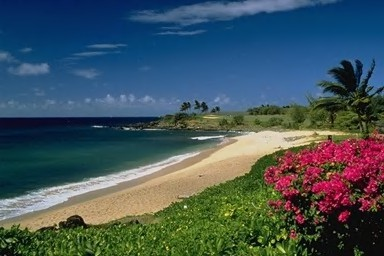
\includegraphics[width=.32\linewidth]{\detokenize{figuras/resultados/2/original-saliencia.png}}
    }
    \subfloat[Original]{
      \includegraphics[width=.32\linewidth]{\detokenize{figuras/resultados/2/original2-saliencia.png}}
    }
    \subfloat[Imagem gerada]{
      \includegraphics[width=.32\linewidth]{\detokenize{figuras/resultados/2/resultado-saliencia.png}}
    }
 \end{center}
 \caption[Geração artificial utilizando o método de \emph{saliência} em duas imagens da classe \textit{Beach} da base de imagens Corel-1000. Detalhes salientes da imagem (b) aparecem sobrepostos à imagem (a) na imagem resultante (c).]{Geração artificial utilizando o método de \emph{saliência} em duas imagens da classe \textit{Beach} da base de imagens Corel-1000. Detalhes salientes da imagem (b) aparecem sobrepostos à imagem (a) na imagem resultante (c). \\ \textit{Fonte:~Elaborado pela autora.}}
 \label{fig:resultados:2:saliencia}
\end{figure}


\item \textbf{Conversão em escala de cinza}: todos os métodos de conversão em escala de cinza foram testados. O método \emph{Luma} resultou em melhor \textit{F1-Score}.

\item \textbf{Extração de características}: todos os métodos para extração foram testados. O método CCV destacou-se como o melhor método para extrair as características que melhor diferenciam essas classes.

\item \textbf{Classificação}: o classificador KNN com $K=1$ foi utilizado.
\end{enumerate}

%-------------------------------------------------------------------------------
\subsubsection*{Resultados}

A combinação dos métodos \emph{Luma} e CCV resultou em melhores valores de \textit{F1-Score}. Como pode ser visto na Tabela \ref{tab:resultados:2:melhor}, diversos métodos de geração artificial de imagens obtiveram resultados melhores que o SMOTE, e na sua maioria maiores do que a base desbalanceada. Destacam-se os métodos de \emph{mistura saliente}, \emph{aguçamento} e a combinação de todos os métodos.

%Na Figura \ref{fig:resultados:2:melhor} é possível verificar o \textit{boxplot} dos \textit{F1-Scores} para as classes desbalanceadas, rebalanceadas com SMOTE após a extração de características e rebalanceadas com os métodos de geração artificial como primeiro passo do \textit{pipeline}.

% \begin{figure}[!htbp]
%   \begin{center}
%\includegraphics[width=\linewidth]{\detokenize{figuras/resultados/2/BIC_Luminance_praia-montanha.png}}
%   \end{center}
%   \caption[Boxplot das classes \textit{Beach} e \textit{Mountain} para a conversão em escala de cinza com\emph{Luminância'} e BIC como método de extração de características.]{Boxplot das classes \textit{Beach} e \textit{Mountain} para a conversão em escala de cinza com\emph{Luminância'} e BIC como método de extração de características. \\ \textit{Fonte:~Elaborado pela autora.}}
%   \label{fig:resultados:2:melhor}
% \end{figure}

\begin{table}[!htbp]
\begin{center}
\caption{Resultados de \textit{F1-Score} para as classes \textit{Beach} e \textit{Mountain}, utilizando \emph{Luma} como método para conversão em escala de cinza e CCV para extração de características. As gerações com aguçamento e saliência obtiveram os melhores resultados.}
\label{tab:resultados:2:melhor}
\begin{tabular}{|l|c|c|}
\hline
\textbf{\emph{Luma} \& CCV} & \textbf{Média}     & \textbf{Desvio Padrão} \\ \hline
   Todos        & \textbf{66.015325} & 5.621643  \\ \hline
  Aguçamento    & \textbf{66.684300} & 5.619944  \\ \hline
  Borramento    & 62.186430 & 6.509084  \\ \hline
  Composição 16 & 63.225965 & 7.920787  \\ \hline
  Composição 4  & 63.824235 & 5.621168  \\ \hline
  Limiares      & 64.453515 & 6.769440  \\ \hline
  Mistura       & 59.506260 & 6.472903  \\ \hline
  Ruído         & 64.202075 & 7.231610  \\ \hline
  SMOTE Visual  & 59.512530 & 7.737273  \\ \hline
  Saliência     & \textbf{66.260870} & 5.732209  \\ \hline
 SMOTE          & 65.531135 & 4.714502  \\ \hline
Desbalanceado   & 59.640090 & 8.675836  \\ \hline
\end{tabular}
\end{center}
\end{table}

%-------------------------------------------------------------------------------
\subsubsection*{Discussão}

A operação de \emph{aguçamento} realça as bordas dos elementos da imagem. Enquanto isso, o método de extração de características CCV classifica os pixels dependendo do tamanho desses componentes. Possivelmente definir melhor as regiões da imagem pode ter auxiliado o sistema de reconhecimento.

De acordo com o teste HSD de Tukey realizado, foi encontrado $\textit{p-value} = 0.0003$ na comparação da base desbalanceada com a base rebalanceada utilizando o método SMOTE e $\textit{p-value} = 0.0000$ com a geração artificial. Isso indica que ambos os métodos obtiveram relevância estatística quando comparados à base desbalanceada. Porém, ao comparar o SMOTE com a geração artificial, o teste resultou em $\textit{p-value} = 0.7122$. Tal valor indica que não há diferença significativa entre os métodos SMOTE e os métodos de geração artificial de imagens.

%%%%%%%%%%%%%%%%%%%%%%%%%%%%%%%%%%%%%%%%%%%%%%%%%%%%%%%%%%%%%%%%%%%%%%%%%%%%%%%%
% \FloatBarrier
\subsection{Experimento 3: multiclasses}

Os dois experimentos anteriores analisaram o rebalanceamento de apenas duas classes. Este experimento apresenta a geração artificial de imagens aplicada a três bases multiclasses: Corel-1000, Caltech101-600 e Produce-1400. Seus resultados são discutidos individualmente.

As bases são originalmente balanceadas, portanto a cada combinação dos \textit{folds}, uma classe é considerada minoritária e três dos seus \textit{folds} são descartados. Restando, dessa forma, um para treino e um para teste. Isso permitiu testar as bases como desbalanceadas.

\subsubsection{Base de imagens Corel}
\label{subsec:corel}

\subsubsubsection*{Protocolo}

\begin{enumerate}
\item \textbf{Imagens originais}: esse experimento foi realizado com a base de imagens Corel-1000, composta por fotografias que representam 10 classes: tribos africanas, praia, construções, ônibus, dinossauros, flores, elefantes, cavalos, montanhas e tipos de comidas \cite{Wang2001}. Para fins de exemplificação, são apresentadas imagens que representam essas classes na Figura \ref{fig:resultados:3:base}.

\begin{figure}[!htbp]
  \begin{center}
    \includegraphics[width=\linewidth]{\detokenize{figuras/quantizacao/fig_COREL_dataset.jpg}}
\end{center}
\caption[Base de imagens Corel-1000. Essa base é composta por fotografias que representam 10 classes: tribos africanas, praia, construções, ônibus, dinossauros, flores, elefantes, cavalos, montanhas e tipos de comidas.]{Base de imagens Corel-1000 \cite{Wang2001}. Essa base é composta por fotografias que representam 10 classes: tribos africanas, praia, construções, ônibus, dinossauros, flores, elefantes, cavalos, montanhas e tipos de comidas. \\ \textit{Fonte:~\citeonline{Ponti2016}.}}
\label{fig:resultados:3:base}
\end{figure}

\item \textbf{Desbalanceamento}: realizaram-se 200 combinações de desbalanceamento dos 5 \textit{folds} para as 10 classes.

\item \textbf{Método para geração artificial}: o método que atingiu o maior \textit{F1-Score} de geração artificial foi a \emph{mistura}. Por esse motivo, ela está exemplificada na Figura \ref{fig:resultados:3.1:mistura}.

\begin{figure}[!htbp]
  \begin{center}
    \subfloat[Original]{
      \includegraphics[width=.32\linewidth]{\detokenize{figuras/resultados/3/original-mistura.png}}
    }
    \subfloat[Original]{
      \includegraphics[width=.32\linewidth]{\detokenize{figuras/resultados/3/original2-mistura.png}}
    }
    \subfloat[Imagem gerada]{
      \includegraphics[width=.32\linewidth]{\detokenize{figuras/resultados/3/resultado-mistura.png}}
    }
\end{center}
\caption[Geração artificial de \emph{mistura} para imagens da base Corel-1000. A imagem resultante (c) apresenta uma mistura das imagens (a) e (b).]{Geração artificial de \emph{mistura} para imagens da base Corel-1000. A imagem resultante (c) apresenta uma mistura das imagens (a) e (b). \\ \textit{Fonte:~Elaborado pela autora.}}
\label{fig:resultados:3.1:mistura}
\end{figure}

\item \textbf{Conversão em escala de cinza}: todos os métodos foram testados e o método \textit{Gleam} obteve os melhores resultados.

\item \textbf{Extração de características}: dada a combinação de todos os métodos, o LBP se sobressaiu entre eles.

\item \textbf{Classificação}: KNN com $K=1$ foi o classificador utilizado.
\end{enumerate}

%-------------------------------------------------------------------------------
\subsubsubsection*{Resultados}

Ao realizar o experimento com as 10 classes da base Corel-1000, a combinação de \emph{Gleam} para conversão em escala de cinza; e LBP como método de extração de características, resultou em melhores \textit{F1-Scores}. A Tabela \ref{tab:resultados:3.1} apresenta a média e o desvio padrão dos \textit{F1-Scores} encontrados nesse experimento. Note que a geração artificial com o método \emph{mistura} obteve \textit{F1-Score} similar ao SMOTE.

\begin{table}[!htbp]
\begin{center}
\caption{Resultados de \textit{F1-Score} para as 10 classes da Corel-1000, utilizando \emph{Gleam} como método para conversão em escala de cinza e LBP para extração de características. A geração artificial com o método \emph{mistura} obteve \textit{F1-Score} similar ao SMOTE.}
\label{tab:resultados:3.1}
\begin{tabular}{|l|c|c|}
\hline
\textbf{\emph{Gleam} \& LBP} & \textbf{Média}     & \textbf{Desvio Padrão} \\ \hline
   Todos        &  61.216388 &  2.205391  \\ \hline
  Aguçamento    &  61.098384 &  2.275732  \\ \hline
  Borramento    &  60.369376 &  2.254895  \\ \hline
  Composição 16 &  60.630235 &  2.212156  \\ \hline
  Composição 4  &  60.568624 &  2.254904  \\ \hline
  Limiares      &  61.296003 &  2.101686  \\ \hline
  Mistura       &  \textbf{61.366671} &  2.225635  \\ \hline
  Ruído         &  60.825884 &  2.358098  \\ \hline
  SMOTE Visual  &  60.886122 &  2.321783  \\ \hline
  Saliência     &  61.050988 &  2.271443  \\ \hline
 SMOTE          &  \textbf{61.368896} &  2.148675  \\ \hline
Desbalanceado   &  60.362256 &  2.290263  \\ \hline
\end{tabular}
\end{center}
\end{table}

%-------------------------------------------------------------------------------
\subsubsubsection*{Discussão}

O método de rebalancemento utilizando a \emph{mistura} de duas imagens acaba por modificar as texturas das imagens. O método de extração de características LPP obteve melhor desempenho e a operação de \emph{mistura} melhor definiu as classes minoritárias.

O rebalanceamento com o método de \emph{mistura} e com o SMOTE tiveram um desempenho quase idêntico (i.e. $\textit{p-value} = 0.9948$). Mas apesar dos \textit{F1-Scores} também parecerem similares à base desbalanceada, o teste HSD de Tukey confirmou que há diferença estatística significante entre eles ($\textit{p-value} = 0.0$). Dessa forma, tanto o SMOTE quanto a geração artificial rebalancearam a base satisfatoriamente.

%%%%%%%%%%%%%%%%%%%%%%%%%%%%%%%%%%%%%%%
\subsubsection{Base de imagens Caltech101-600}

\subsubsubsection*{Protocolo}

\begin{enumerate}
\item \textbf{Imagens originais}: foi utilizada a base Caltech101-600 \cite{Fei-Fei2007}. Desta base, foi utilizado um conjunto de seis classes balanceadas: aviões, bonsais, candelabros, tartarugas, motocicletas e relógios. Imagens que representam essas classes são apresentadas na Figura \ref{fig:resultados:3.2:base}.

\begin{figure}[!htbp]
  \begin{center}
    \includegraphics[width=0.8\linewidth]{\detokenize{figuras/quantizacao/fig_Caltech101_dataset.jpg}}
\end{center}
\caption[Conjunto de seis classes balanceadas: aviões, bonsais, candelabros, tartarugas, motocicletas e relógios da base de imagens Caltech101-600.]{Conjunto de seis classes balanceadas: aviões, bonsais, candelabros, tartarugas, motocicletas e relógios da base de imagens Caltech~\cite{Fei-Fei2007}. \\
\textit{Fonte:~\citeonline{Ponti2016}.}}
\label{fig:resultados:3.2:base}
\end{figure}

\item \textbf{Desbalanceamento}: 120 combinações de 5 \textit{folds} para as 6 classes foram testadas. Cobrindo, assim, todas as possibilidades para garantir que cada imagem pudesse pertencer a majoritária, minoritária, treino, teste ou não ser utilizada na classificação.

\item \textbf{Método para geração artificial}: o melhor resultado em termos de geração artificial foi utilizando todas as gerações. A Figura   \ref{fig:resultados:3.2:limiares} apresenta um exemplo da geração com \emph{mistura de limiares}, uma das possíveis gerações artificiais.

  \begin{figure}[!htbp]
    \begin{center}
    \subfloat[Original]{
      \includegraphics[height=2cm,keepaspectratio]{\detokenize{figuras/resultados/3/original-limiares.png}}
    }
    \subfloat[Original]{
      \includegraphics[height=2cm,keepaspectratio]{\detokenize{figuras/resultados/3/original2-limiares.png}}
    }
    \subfloat[Imagem gerada]{
      \includegraphics[height=2cm,keepaspectratio]{\detokenize{figuras/resultados/3/resultado-limiares.png}}
    }
  \end{center}
  \caption[Exemplo de uma geração artificial utilizando o método de \emph{mistura limiarizada} para a base Caltech101-600.]{Exemplo de uma geração artificial utilizando o método de \emph{mistura limiarizada} para a base de imagens Caltech101-600. \\ \textit{Fonte:~Elaborado pela autora.}}
  \label{fig:resultados:3.2:limiares}
  \end{figure}

\item \textbf{Conversão em escala de cinza}: todos os métodos foram testados. O que obteve melhores resultados foi o \textit{Intensidade'}.
\item \textbf{Extração de características}: de todos os métodos foram testados, o HOG foi o melhor método de extração de características.
\item \textbf{Classificação}: classificador KNN com $K=1$.
\end{enumerate}

%-------------------------------------------------------------------------------
\subsubsubsection*{Resultados}

Considerando que essa base possui 6 classes, 120 sub-experimentos foram necessários para cobrir todas as possibilidades de desbalanceamento. Os resultados de tais experimentos são apresentados na Tabela \ref{tab:resultados:3.2}. É possível notar que tanto o SMOTE quanto a geração artificial utilizando todos os métodos obtiveram um \textit{F1-Score} melhor que a versão desbalanceada.

\begin{table}[!htbp]
\begin{center}
\caption{Resultados do experimento com a base Caltech101-600. É possível notar que tanto o SMOTE quanto a geração artificial utilizando todos os métodos obtiveram um \textit{F1-Score} melhor que a versão desbalanceada.}
\label{tab:resultados:3.2}
\begin{tabular}{|l|c|c|}
\hline
\textbf{\emph{Intensidade'} \& HOG} & \textbf{Média} & \textbf{Desvio Padrão} \\ \hline
   Todos        &  \textbf{77.591493} &  3.387543  \\ \hline
  Aguçamento    &  76.982412 &  3.482750  \\ \hline
  Borramento    &  75.736587 &  3.812333  \\ \hline
  Composição 16 &  75.742438 &  3.823391  \\ \hline
  Composição 4  &  75.787022 &  3.794589  \\ \hline
  Limiares      &  76.785628 &  3.652596  \\ \hline
  Mistura       &  77.186702 &  3.382386  \\ \hline
  Ruído         &  77.344959 &  3.664212  \\ \hline
  SMOTE Visual  &  75.486170 &  4.405685  \\ \hline
  Saliência     &  76.587268 &  3.600158  \\ \hline
 SMOTE          &  \textbf{77.755417} &  3.529355  \\ \hline
Desbalanceado   &  75.732382 &  3.833682  \\ \hline
\end{tabular}
\end{center}
\end{table}

%-------------------------------------------------------------------------------
\subsubsubsection*{Discussão}

A combinação aleatória uniforme de todos os métodos obteve um \textit{F1-Score} melhor do que cada método individualmente. Com o teste \textit{post-hoc} HSD de Tukey tem-se um indício de que os resultados do SMOTE e da geração artificial utilizando todos os métodos não possuem diferença estatística. Isso porque resultaram em $\textit{p-value} = 0.9333$. Porém, entre o desbalanceado e o SMOTE ou a geração obteve-se $\textit{p-value} < 0.0$. O que indica que todos os métodos de rebalanceamento foram satisfatórios para a base Caltech101-600.

%%%%%%%%%%%%%%%%%%%%%%%%%%%%%%%%%%%%%%%
\subsubsection{Base de imagens Produce}

\subsubsubsection*{Protocolo}

\begin{enumerate}
\item \textbf{Imagens originais}: base de imagens Produce-1400, composta por imagens de vegetais e frutas tropicais \cite{Rocha2010}. Possuem fundo similar mas muitas mudanças na iluminação, no número de objetos e na escala. Amostras das imagens dessa base são apresentadas na Figura \ref{fig:resultados:3.3:base}. Essa base contem 14 classes e um total de 1400 imagens.

\begin{figure}[!htbp]
  \begin{center}
    \includegraphics[width=\linewidth]{\detokenize{figuras/quantizacao/fig_Produce_dataset.jpg}}
\end{center}
\caption[Base de imagens Produce-1400, composta por imagens de vegetais e frutas tropicais. A base possui classes com fundo similar, porém com variações na iluminação, número de objetos, cor e escala.]{Base de imagens Produce-1400, composta por imagens de vegetais e frutas tropicais \cite{Rocha2010}. A base possui classes com fundo similar, porém com variações na iluminação, número de objetos, cor e escala. \\ \textit{Fonte:~\citeonline{Ponti2016}.}}
\label{fig:resultados:3.3:base}
\end{figure}

\item \textbf{Desbalanceamento}: considerando que a base Produce-1400 é balanceada, 280 combinações dos 5 \textit{folds} das 14 classes foram testadas. Dessa forma todas as classes tiveram chance de serem a classe minoritária e, assim, rebalanceadas.
\item \textbf{Método para geração artificial}: o melhor método de geração para a base Produce-1400 foi a \emph{mistura}, exemplificada na Figura \ref{fig:resultados:3.3:mistura}.

  \begin{figure}[!htbp]
    \begin{center}
    \subfloat[Original]{
      \includegraphics[width=.32\linewidth]{\detokenize{figuras/resultados/3/original-mistura-produce.png}}
    }
    \subfloat[Original]{
      \includegraphics[width=.32\linewidth]{\detokenize{figuras/resultados/3/original2-mistura-produce.png}}
    }
    \subfloat[Imagem gerada]{
      \includegraphics[width=.32\linewidth]{\detokenize{figuras/resultados/3/resultado-mistura-produce.png}}
    }
    \end{center}
    \caption[Exemplo de geração artificial utilizando a \emph{mistura} de duas imagens para a base Produce.]{Exemplo de geração artificial utilizando a \emph{mistura} de duas imagens para a base Produce-1400. \\ \textit{Fonte:~Elaborado pela autora.}}
    \label{fig:resultados:3.3:mistura}
  \end{figure}

\item \textbf{Conversão em escala de cinza}: todas as combinações de métodos foram testadas. \emph{Luma} destacou-se como o melhor método para converter a imagem em escala de cinza.
\item \textbf{Extração de características}: todos os métodos foram testados. O LBP obteve os melhores resultados como método para extrair as características.
\item \textbf{Classificação}: classificador KNN com $K=1$.
\end{enumerate}

%-------------------------------------------------------------------------------
\subsubsubsection*{Resultados}

A Tabela \ref{tab:resultados:3.3} apresenta a média e o desvio padrão dos \textit{F1-Scores} encontrados nos 280 sub-experimentos para a base Produce-1400. Esses cobrem todas as possibilidades de desbalanceamento. O método de \emph{mistura} resultou no melhor \textit{F1-Score}.

\begin{table}[!htbp]
\begin{center}
\caption{Resultados de \textit{F1-Scores} para a base de imagens Produce-1400. O método \emph{mistura} apresentou-se como o melhor.}
\label{tab:resultados:3.3}
\begin{tabular}{|l|c|c|}
\hline
\textbf{\emph{Luma} \& LBP} & \textbf{Média}     & \textbf{Desvio Padrão} \\ \hline
   Todos        &  91.682606 &  1.985052  \\ \hline
  Aguçamento    &  91.463371 &  2.039631  \\ \hline
  Borramento    &  91.493838 &  2.022884  \\ \hline
  Composição 16 &  91.476496 &  2.037559  \\ \hline
  Composição 4  &  91.478369 &  2.021889  \\ \hline
  Limiares      &  91.843197 &  1.934367  \\ \hline
  Mistura       &  \textbf{91.985465} &  1.949951  \\ \hline
  Ruído         &  91.489904 &  2.028988  \\ \hline
  SMOTE Visual  &  91.473853 &  2.031678  \\ \hline
  Saliência     &  91.772214 &  2.006734  \\ \hline
 SMOTE          &  91.869133 &  1.952464  \\ \hline
Desbalanceado   &  91.489904 &  2.028988  \\ \hline
\end{tabular}
\end{center}
\end{table}

%-------------------------------------------------------------------------------
\subsubsubsection*{Discussão}

Assim como no experimento da Seção \ref{subsec:corel}, a combinação de extração de características com o método LBP e o rebalanceamento com a operação de \emph{mistura} favoreceu a classificação desse cenário. O teste \textit{post-hoc} HSD de Tukey indicou que há relevância estatística entre os \textit{F1-Scores} da base desbalanceada quando comparada com o rebalanceamento utilizando o método de \emph{mistura} ($ \textit{p-value} = 0.0087$). Mas comparado com SMOTE, o $\textit{p-value} = 0.0607$ indica que não há diferença significante entre ele e a versão original. Ainda assim, o teste resultou em $\textit{p-value} = 0.7658$ para a comparação entre o SMOTE e a geração artificial, indicando que não há significância entre os dois. De qualquer forma, tais resultados indicam que a geração artificial de \emph{mistura} obteve resultado significativo.

%%%%%%%%%%%%%%%%%%%%%%%%%%%%%%%%%%%%%%%%%%%%%%%%%%%%%%%%%%%%%%%%%%%%%%%%%%%%%%%%
% \FloatBarrier
\subsection{Experimento 4: classes naturalmente desbalanceadas}

Os experimentos anteriores foram realizados em bases já balanceadas, com o desbalancemento sendo provocado. Este experimento utiliza duas combinações de classes de imagens naturalmente desbalanceadas.

% Os sub-experimentos foram realizados de forma diferente que os anteriores. Isso foi realizado indicando que o número de imagens faltantes são do \textit{fold} que não seria utilizado, caso fosse o caso de bases balanceadas (experimentos anteriores). Ou seja, todas as classes ainda continuam com \textit{5-folds} cada.

\subsubsection{Duas classes desbalanceadas: \textit{Eiffel Tower} e \textit{Rome antica}}

% Esse experimento aponta os resultados para duas classes naturalmente desbalanceadas.

\subsubsubsection*{Protocolo}

\begin{enumerate}
\item \textbf{Imagens originais}: as classes utilizadas para esse experimento foram \textit{Eiffel Tower} com 1607 imagens, e \textit{Rome antica} com apenas 125 imagens \cite{Hu2013}. Essas classes possuem fundo similar, mas formas distintas.

\begin{figure}[!htbp]
  \begin{center}
    \subfloat[\textit{Eiffel Tower}]{
      \includegraphics[height=5.5cm,keepaspectratio]{\detokenize{figuras/resultados/4/class13-1.png}}
    }
    \subfloat[\textit{Rome antica}]{
      \includegraphics[height=5.5cm,keepaspectratio]{\detokenize{figuras/resultados/4/class41-2.png}}
    }
\end{center}
\caption[Imagens das classes naturalmente desbalanceadas \textit{Eiffel Tower}, com 1607 imagens, e \textit{Rome antica}, com apenas 125 imagens.]{Imagens das classes naturalmente desbalanceadas \textit{Eiffel Tower}, com 1607 imagens, e \textit{Rome antica}, com apenas 125 imagens. \\ \textit{Fonte:~\citeonline{Hu2013}.}}
\label{fig:resultados:4.1:base}
\end{figure}

\item \textbf{Desbalanceamento}: natural da base. A classe minoritária é a \textit{Rome antica} com 125 imagens. Dessa forma, a cada combinação dos \textit{folds}, $1607 - 125 = 1482$ imagens foram geradas para rebalancear a base.

\item \textbf{Método para geração artificial}: todas as gerações foram testadas, a que obteve melhor resultado foi a \emph{mistura}. Essa geração está exemplificada na Figura \ref{fig:resultados:4.1:geracao}.


  \begin{figure}[!htbp]
    \begin{center}
    \subfloat[Original]{
      \includegraphics[height=3.8cm,keepaspectratio]{\detokenize{figuras/resultados/4/original-mistura.png}}
    }
    \subfloat[Original]{
      \includegraphics[height=3.8cm,keepaspectratio]{\detokenize{figuras/resultados/4/original2-mistura.png}}
    }
    \subfloat[Imagem gerada]{
      \includegraphics[height=3.8cm,keepaspectratio]{\detokenize{figuras/resultados/4/resultado-mistura.png}}
    }
    \end{center}
    \caption[Exemplo de geração artificial utilizando a \emph{mistura} de duas imagens da classe \textit{Rome antica}.]{Exemplo de geração artificial utilizando a \emph{mistura} de duas imagens da classe \textit{Rome antica}. \\ \textit{Fonte:~Elaborado pela autora.}}
    \label{fig:resultados:4.1:geracao}
  \end{figure}


\item \textbf{Conversão em escala de cinza}: todos os métodos foram testados. O que obteve melhor \textit{F1-Score} foi o MSB.
\item \textbf{Extração de características}: de todos os métodos para extração testados, o HOG obteve os melhores resultados. Isso confirma que as classes são diferenciadas pela sua forma.
\item \textbf{Classificação}: KNN com $K=1$.
\end{enumerate}

%-------------------------------------------------------------------------------
\subsubsubsection*{Resultados}

O rebalanceamento foi realizado de forma a balancear a classe minoritária \textit{Rome antica}. A Tabela \ref{tab:resultados:4.1} apresenta os resultados de tal rebalanceamento. Nela estão os resultados de média e desvio padrão do rebalanceamento realizado com a combinação dos \textit{folds} das duas classes. O método que obteve maior valor de \textit{F1-Score} foi o de geração artificial com o método de \emph{mistura} de duas imagens.

\begin{table}[!htbp]
\begin{center}
\caption{Resultados de \textit{F1-Score} para as classes \textit{Eiffel Tower} e \textit{Rome antica}, naturalmente desbalanceadas. O método \textit{mistura} destacou-se como o melhor método para rebalanceamento dessas classes.}
\label{tab:resultados:4.1}
\begin{tabular}{|l|c|c|}
\hline
\textbf{MSB \& HOG} & \textbf{Média}     & \textbf{Desvio Padrão} \\ \hline
   Todos        &  88.616130 &  1.952745  \\ \hline
  Aguçamento    &  98.345625 &  1.755180  \\ \hline
  Borramento    &  97.173480 &  2.760269  \\ \hline
  Composição 16 &  97.206953 &  2.712589  \\ \hline
  Composição 4  &  97.301088 &  2.381761  \\ \hline
  Limiares      &  98.628050 &  1.142830  \\ \hline
  Mistura       &  \textbf{99.112148} &  0.837440  \\ \hline
  Ruído         &  91.499965 &  1.762218  \\ \hline
  SMOTE Visual  &  82.963755 &  2.678785  \\ \hline
  Saliência     &  98.246915 &  1.526565  \\ \hline
 SMOTE          &  98.471765 &  0.788747  \\ \hline
Desbalanceado   &  97.173480 &  2.760269  \\ \hline
\end{tabular}
\end{center}
\end{table}

%-------------------------------------------------------------------------------
\subsubsubsection*{Discussão}

O método de extração de características HOG calcula a frequência da ocorrência da orientação dos gradientes em janelas da imagem. O método de rebalanceamento utilizando a mistura de duas imagens se sobressaiu, possivelmente devido a modificar as texturas das imagens.

Apesar de valores de \textit{F1-Score} próximos, de acordo com o teste \textit{post-hoc} de Tukey, foi encontrado $\textit{p-value} = 0.0030$ para a base desbalanceada quando comparado com o rebalanceamento com SMOTE. Isso indica que há significância estatística relevante entre eles. O teste também indicou que há significância entre a base desbalanceada e ela rebalanceada com a geração artificial ($\textit{p-value} = 0.0000$). Porém, se comparados o SMOTE e a geração artificial temos $\textit{p-value} = 0.2255$, indicando que não há diferença significante.

%-------------------------------------------------------------------------------
\subsubsection{Multiclasses desbalanceadas: \textit{Trafalgar Square}, \textit{Madeleine Church} e \textit{Pantheon}}
% Esse experimento apresenta os resultados encontrados ao utilizar três classes naturalmente desbalanceadas.

\subsubsubsection*{Protocolo}
\begin{enumerate}

\item \textbf{Imagens originais}: foram utilizadas \textit{Trafalgar Square}, \textit{Madeleine Church} e \textit{Pantheon} \cite{Hu2013}. Essas classes são apresentadas na Figura \ref{fig:resultados:4.2:base}. Elas contêm tanto imagens parecidas (difícil classificação), quanto imagens bem divergentes (fácil diferenciação).

\begin{figure}[!htbp]
  \begin{center}
    \subfloat[Trafalgar Square]{
      \includegraphics[height=3.8cm,keepaspectratio]{\detokenize{figuras/resultados/4/trafalgar.png}}
    }
    \subfloat[Madeleine Church]{
      \includegraphics[height=3.8cm,keepaspectratio]{\detokenize{figuras/resultados/4/madeleine.png}}
    }
    \subfloat[Pantheon]{
      \includegraphics[height=3.8cm,keepaspectratio]{\detokenize{figuras/resultados/4/pantheon.png}}
    }
\end{center}
\caption[Imagens representativas das classes \textit{Trafalgar Square}, \textit{Madeleine Church} e \textit{Pantheon}. Elas contêm tanto imagens parecidas (difícil classificação), quanto imagens bem divergentes (fácil diferenciação).]{Imagens representativas das classes \textit{Trafalgar Square}, \textit{Madeleine Church} e \textit{Pantheon}. Elas contêm tanto imagens parecidas (difícil classificação), quanto imagens bem divergentes (fácil diferenciação). \\ \textit{Fonte:~\citeonline{Hu2013}.}}
\label{fig:resultados:4.2:base}
\end{figure}

\item \textbf{Desbalanceamento}: natural da base. A classe \textit{Trafalgar Square} contém 132 imagens, a \textit{Madeleine Church} 316 e a \textit{Pantheon} 23. Para rebalancear foram necessárias $316 - 132 = 147$ imagens para a \textit{Trafalgar Square} e $316 - 23 = 234$ para a classe \textit{Pantheon}.

\item \textbf{Método para geração artificial}: todas as gerações foram testadas, mas a melhor foi a de \emph{composição} de quatro imagens, retratada na Figura \ref{fig:resultados:4.2:geracao}.

\begin{figure}[!htbp]
  \begin{center}
  \subfloat{
    \includegraphics[width=.5\linewidth]{\detokenize{figuras/resultados/4/resultado-composicao.png}}
  }
  \caption[Exemplo de geração artificial realizada com a \emph{composição} de quatro imagens para a classe \textit{Pantheon}.]{Exemplo de geração artificial realizada com a \emph{composição} de quatro imagens para a classe \textit{Pantheon}. \\ \textit{Fonte:~Elaborado pela autora.}}
  \label{fig:resultados:4.2:geracao}
  \end{center}
\end{figure}

\item \textbf{Conversão em escala de cinza}: de todos os métodos foram testados, o melhor para essas imagens foi o \emph{Gleam}.
\item \textbf{Extração de características}: todos os métodos para extração foram testados, mas o HOG obteve melhores resultados.
\item \textbf{Classificação}: KNN com $K=1$ foi o classificador utilizado.
\end{enumerate}

%-------------------------------------------------------------------------------
\subsubsubsection*{Resultados}

Os melhores métodos para extração e conversão em escala de cinza foram HOG e \emph{Gleam}, respectivamente. O método de geração artificial de imagens que obteve o melhor \textit{F1-Score} foi a \emph{composição} de quatro imagens e a Tabela \ref{tab:resultados:4.2} apresenta tais resultados. O método SMOTE piorou significativamente a classificação, mas a geração artificial ficou muito similar a classificação sem gerar imagem nenhuma.

\begin{table}[!htbp]
\begin{center}
\caption{Resultados utilizando os métodos HOG e \textit{Gleam} para as classes \textit{Trafalgar Square}, \textit{Madeleine Church} e \textit{Pantheon}. O método SMOTE piorou significativamente a classificação, mas a geração artificial ficou muito similar a classificação sem gerar imagem nenhuma.}
\label{tab:resultados:4.2}
\begin{tabular}{|l|c|c|}
\hline
\textbf{\emph{Gleam} \& HOG} & \textbf{Média}     & \textbf{Desvio Padrão} \\ \hline
   Todos        &  57.285167 &  6.383771  \\ \hline
  Aguçamento    &  69.726448 &  8.069939  \\ \hline
  Borramento    &  70.621480 &  8.314352  \\ \hline
  Composição 16 &  70.478478 &  8.366100  \\ \hline
  Composição 4  &  \textbf{70.837125} &  7.811876  \\ \hline
  Limiares      &  67.965067 &  5.699239  \\ \hline
  Mistura       &  65.644708 &  6.112751  \\ \hline
  Ruído         &  60.777810 &  8.257640  \\ \hline
  SMOTE Visual  &  53.912270 &  7.907406  \\ \hline
  Saliência     &  67.584110 &  6.236710  \\ \hline
 SMOTE          &  62.322870 &  5.726037  \\ \hline
Desbalanceado   &  70.621480 &  8.314352  \\ \hline
\end{tabular}
\end{center}
\end{table}

%-------------------------------------------------------------------------------
\subsubsubsection*{Discussão}

Utilizando o teste \textit{post-hoc} de Tukey, foi encontrado $\textit{p-value} = 0.0$ para a base desbalanceada versus o rebalanceamento com SMOTE. Isso indica que há significância estatística relevante entre eles. O teste também indicou que não há significância entre a base desbalanceada e ela rebalanceada com a geração artificial ($\textit{p-value} = 0.9858$). Além disso, se comparados o SMOTE e a geração artificial temos $\textit{p-value} = 0.0$, indicando que há diferença significante. Ou seja, o método SMOTE foi significativamente pior que a base original e o método de geração artificial teve uma melhora não estatisticamente significativa.

%%%%%%%%%%%%%%%%%%%%%%%%%%%%%%%%%%%%%%%%%%%%%%%%%%%%%%%%%%%%%%%%%%%%%%%%%%%%%%%%
% \FloatBarrier
\subsection{Experimento 5: classes com muitas imagens}

Por fim, este experimento foi realizado com duas classes contendo uma grande quantidade de imagens.

\subsubsection{Classes balanceadas, distintas e com grande número de imagens}
% Esse experimento relata os resultados encontrados para duas classes balanceadas, com grande número de imagens cada.

\subsubsubsection*{Protocolo}

\begin{enumerate}
\item \textbf{Imagens originais}: classes \textit{Deer} e \textit{Ship}, cada uma com 5000 imagens cada \cite{Krizhevsky2009}. Essas imagens possuem dimensão de apenas 32x32 pixels, o que dificulta a representatividade da extração de características (ver Figura \ref{fig:resultados:5.1:base}).

\begin{figure}[!htbp]
  \begin{center}
  \subfloat[\textit{Deer}]{
    \includegraphics[width=.3\linewidth]{\detokenize{figuras/resultados/5/cervo.png}}
  }
  \subfloat[\textit{Ship}]{
    \includegraphics[width=.3\linewidth]{\detokenize{figuras/resultados/5/navio.png}}
  }
  \end{center}
  \caption[Imagens representativas das classes \textit{Deer} e \textit{Ship}. São imagens em baixa resolução (32x32 pixels), o que dificulta o seu processamento e posterior clasificação.]{Imagens representativas das classes \textit{Deer} e \textit{Ship}. São imagens em baixa resolução (32x32 pixels), o que dificulta o seu processamento e posterior clasificação. \\ \textit{Fonte:~\citeonline{Krizhevsky2009}}.}
  \label{fig:resultados:5.1:base}
\end{figure}

\item \textbf{Desbalanceamento}: são classes balanceadas. Por conta disso, todas as combinações dos 5 \textit{folds} foram testadas.

\item \textbf{Método para geração artificial}: a operação de \textit{aguçamento} obteve maiores valores de \textit{F1-Score} dentre todos os métodos de rebalanceamento.

%
%   \begin{figure}[!htbp]
%     \begin{center}
%     \subfloat[Original]{
%       \includegraphics[height=3.5cm,keepaspectratio]{\detokenize{figuras/resultados/5/original-agucamento.png}}
%     }
%     \subfloat[Aguçcamento]{
%       \includegraphics[height=3.5cm,keepaspectratio]{\detokenize{figuras/resultados/5/resultado-agucamento.png}}
%     }
%     \caption[Exemplo de geração artificial utilizando a \emph{mistura} de duas imagens para a base Produce-1400.]{Exemplo de geração artificial utilizando a \emph{mistura} de duas imagens para a base Produce-1400. \\ \textit{Fonte:~Elaborado pela autora.}}
%     \label{fig:resultados:5.1:geracao}
%     \end{center}
%   \end{figure}

\item \textbf{Conversão em escala de cinza}: todos os métodos de conversão em escala de cinza foram testados. O que resultou em melhor \textit{F1-Score} foi o \emph{Gleam}.

\item \textbf{Extração de características}: todos os métodos para extração foram testados, mas o método HOG destacou-se como o melhor.

\item \textbf{Classificação}: o classificador utilizado foi o KNN com $K=1$.

\end{enumerate}
%-------------------------------------------------------------------------------
\subsubsubsection*{Resultados}

Os resultados encontrados ao rebalancear as classes \textit{Deer} e \textit{Ship} estão apresentados na Tabela \ref{tab:resultados:5.1}. Os rebalanceamentos com imagens artificiais geradas com os métodos \emph{aguçamento} \textit{mistura limiarizada} e \textit{mistura ponderada} apresentaram os melhores resultados.

\begin{table}[!htbp]
\begin{center}
\caption{Resultados de \textit{F1-Score} para as classes \textit{Deer} e \textit{Ship}, utilizando \emph{Gleam} como método para conversão em escala de cinza e HOG para extração de características. As gerações de imagens com \textit{aguçamento}, \textit{mistura limiarizada} e \textit{mistura ponderada} obtiveram os melhores resultados.}
\label{tab:resultados:5.1}
\begin{tabular}{|l|c|c|}
\hline
\textbf{\emph{Gleam} \& HOG} & \textbf{Média}     & \textbf{Desvio Padrão} \\ \hline
   Todos        &  88.939785 &  1.035462  \\ \hline
  Aguçamento    &  \textbf{89.473075} &  0.961293  \\ \hline
  Borramento    &  88.150530 &  1.006920  \\ \hline
  Composição 16 &  88.086065 &  0.987147  \\ \hline
  Composição 4  &  88.360675 &  0.949842  \\ \hline
  Limiares      &  \textbf{89.356875} &  0.942907  \\ \hline
  Mistura       &  \textbf{89.445505} &  0.939809  \\ \hline
  Ruído         &  86.762190 &  1.165064  \\ \hline
  SMOTE Visual  &  88.395965 &  1.081594  \\ \hline
  Saliência     &  88.136675 &  0.988034  \\ \hline
 SMOTE          &  63.183905 &  2.355925  \\ \hline
Desbalanceado   &  88.121310 &  0.985599  \\ \hline
\end{tabular}
\end{center}
\end{table}

%-------------------------------------------------------------------------------
\subsubsubsection*{Discussão}

Considerando que o método HOG calcula a frequência da ocorrência da orientação dos gradientes da imagem, os métodos de rebalanceamento que se destacaram alteraram essa frequência de modo a melhor definir as classes. Ao realizar o teste \textit{post-hoc} de Tukey, foi encontrado $\textit{p-value} = 0.0$ para a base desbalanceada quando comparada com o rebalanceamento com SMOTE. Isso indica que há significância estatística relevante entre eles e também entre a base desbalanceada e ela rebalanceada com a geração artificial ($\textit{p-value} = 0.0006$). Além disso, se comparados o SMOTE e a geração artificial tem-se $\textit{p-value} = 0.0$, indicando que há diferença significante. Assim, os resultados apontam que SMOTE piorou significativamente a classificação, enquanto a geração artificial forneceu uma melhora considerável.

%-------------------------------------------------------------------------------
\subsubsection{Classes balanceadas, similares e com grande número de imagens}
% Esse experimento indica os resultados para duas classes balanceadas, com grande número de imagens cada.

\subsubsubsection*{Protocolo}

\begin{enumerate}
\item \textbf{Imagens originais}: classes \textit{Shark} e \textit{Fish} com 1300 imagens cada \cite{Russakovsky2015}. Essas classes são exemplificadas na Figura \ref{fig:resultados:5.2:base}.

\begin{figure}[!htbp]
  \begin{center}
    \subfloat[\textit{Shark}]{
      \includegraphics[height=4cm,keepaspectratio]{\detokenize{figuras/resultados/5/tubarao.png}}
    }
    \subfloat[\textit{Fish}]{
      \includegraphics[height=4cm,keepaspectratio]{\detokenize{figuras/resultados/5/peixe.png}}
    }
\end{center}
\caption[Imagens das classes \textit{Shark} e \textit{Fish}. Essas classes apresentam fundo similar.]{Imagens das classes \textit{Shark} e \textit{Fish}. Essas classes apresentam fundo similar. \\ \textit{Fonte:~\citeonline{Russakovsky2015}.}}
\label{fig:resultados:5.2:base}
\end{figure}

\item \textbf{Desbalanceamento}: as duas classes estão balanceadas. Assim, esse experimento realizou a combinação dos 5 \textit{folds} de cada classe para testar o rebalanceamento.

\item \textbf{Método para geração artificial}: a \emph{mistura limiarizada} foi o método de geração artificial que obteve maior \textit{F1-Score}, exemplificada na Figura~\ref{fig:resultados:5.2:geracao}.

  \begin{figure}[!htbp]
    \begin{center}
    \subfloat[Original]{
      \includegraphics[height=4cm,keepaspectratio]{\detokenize{figuras/resultados/5/original-limiares.png}}
    }
    \subfloat[Imagem gerada]{
      \includegraphics[height=4cm,keepaspectratio]{\detokenize{figuras/resultados/5/resultado-limiares.png}}
    }
    \end{center}
    \caption[Exemplo de geração artificial utilizando a \emph{mistura limiarizada} de duas imagens para a classe \textit{Fish}. Por se tratarem de imagens com \textit{foreground} facilmente destacado, a combinação de limiares oferece uma mistura interessante dos objetos.]{Exemplo de geração artificial utilizando a \emph{mistura limiarizada} de duas imagens para a classe \textit{Fish}. Por se tratarem de imagens com \textit{foreground} facilmente destacado, a combinação de limiares oferece uma mistura interessante dos objetos. \\ \textit{Fonte:~Elaborado pela autora.}}
    \label{fig:resultados:5.2:geracao}
  \end{figure}

\item \textbf{Conversão em escala de cinza}: todos os métodos de conversão em escala de cinza foram testados. O que resultou em melhor \textit{F1-Score} foi o \emph{Luma}.

\item \textbf{Extração de características}: todos os métodos para extração foram testados, mas o que melhor se destacou foi o LBP.
\item \textbf{Classificação}: KNN com $K = 1$ foi o classificador utilizado.

\end{enumerate}
%-------------------------------------------------------------------------------
%-------------------------------------------------------------------------------
\subsubsubsection*{Resultados}

A Tabela \ref{tab:resultados:shark} apresenta a média e o desvio padrão encontrados ao rebalancear as classes \textit{Shark} e \textit{Fish}. Pode ser verificado que a geração artificial com a \emph{mistura limiarizada} aparenta ser o melhor método para rebalanceá-las.

\begin{table}[!htbp]
\begin{center}
\caption{Resultados de \textit{F1-Score} para as classes \textit{Shark} e \textit{Fish}. A geração artificial com a \emph{mistura limiarizada} apresenta-se como o melhor método para rebalanceá-las.}
\label{tab:resultados:shark}
\begin{tabular}{|l|c|c|}
\hline
\textbf{\emph{Luma} \& LBP} & \textbf{Média}     & \textbf{Desvio Padrão} \\ \hline
   Todos        &  77.128293 &  2.064232  \\ \hline
  Aguçamento    &  76.862198 &  1.786898  \\ \hline
  Borramento    &  73.919025 &  1.942236  \\ \hline
  Composição 16 &  75.435960 &  2.254193  \\ \hline
  Composição 4  &  74.359165 &  1.974563  \\ \hline
  Limiares      &  \textbf{78.330465} &  1.768789  \\ \hline
  Mistura       &  77.381940 &  2.588103  \\ \hline
  Ruído         &  74.094233 &  1.743535  \\ \hline
  SMOTE Visual  &  74.569545 &  1.648100  \\ \hline
  Saliência     &  76.934077 &  2.114528  \\ \hline
 SMOTE          &  78.066890 &  2.107176  \\ \hline
Desbalanceado   &  73.378227 &  2.110355  \\ \hline
\end{tabular}
\end{center}
\end{table}

%-------------------------------------------------------------------------------
\subsubsubsection*{Discussão}

Considerando que as classes \textit{Shark} e \textit{Fish} possuem objetos de cena bem definidos, a limiarização utilizando o \textit{threshold} de OTSU acaba por compor as imagens sem provocar efeitos nessa combinação. Como o LBP utiliza histogramas dos padrões de textura, misturar os padrões dos objetos de cena de uma imagem com os de fundo de outra imagem acabou por melhorar a classificação do sistema.

Como esperado, de acordo com o teste \textit{post-hoc} de Tukey foi encontrado $\textit{p-value} = 0.0$ para a base desbalanceada quando comparada com o SMOTE. Isso indica que há significância estatística relevante entre eles. Tal teste também indicou que há significância entre a base desbalanceada e ela rebalanceada com a geração artificial ($\textit{p-value} = 0.0$). Porém, não há diferença significante na comparação entre o SMOTE e a geração artificial ($\textit{p-value} = 0.8264$). Assim, ambos métodos rebalancearam as classes satisfatoriamente.

%%%%%%%%%%%%%%%%%%%%%%%%%%%%%%%%%%%%%%%%%%%%%%%%%%%%%%%%%%%%%%%%%%%%%%%%%%%%%%%%
% \FloatBarrier
% \subsection{Experimento 6: fine-tunning}
%
% \meutodo{Estou fazendo}

%%%%%%%%%%%%%%%%%%%%%%%%%%%%%%%%%%%%%%%%%%%%%%%%%%%%%%%%%%%%%%%%%%%%%%%%%%%%%%%%
% \begin{figure}[!htbp]
%   \begin{center}
%     \begin{subfigure}{.49\linewidth}
%       \centering
%       \includegraphics[width=\linewidth]{\detokenize{figuras/visualizacao/original.png}}
%     \end{subfigure}
%     \begin{subfigure}{.49\linewidth}
%       \centering
%       \includegraphics[width=\linewidth]{\detokenize{figuras/visualizacao/desbalanceado-fixed.png}}
%     \end{subfigure}
%   \end{center}
%   \caption{Remoção de 50\% das imagens de treino da classe Horse.}
%   \label{fig:desbalanceado}
% \end{figure}

%-------------------------------------------------------------------------------

% Também foi possível notar que algumas operações não provocaram a melhora da classificação. A operação de \emph{adição de ruído} para geração artificial, a posterior extração utilizando CCV e a quantização por MSB, destacou-se como o pior resultado, apresentado na Figura~\ref{fig:resultpior}. Outros casos que não obtiveram o resultado esperado envolveram as operações de \emph{borramento} e de \textit{unsharp masking}.

% Após a realização dos testes, as operações que melhor se destacaram foram: utilizar todas as operações, apenas \emph{mistura} e apenas \emph{composição}. E as operações que resultaram em uma classificação pior do que o uso do SMOTE foram: utilizar apenas \emph{borramento}, ruído ou \textit{unsharp masking}. Com o teste estatístico de Friedman foi possível verificar que o ACC foi o extrator que melhor se beneficiou das características geradas; e CCV e GCH os menos beneficiados. \enlargethispage{-\baselineskip} A Tabela \ref{tab:result} apresenta os \textit{rankings} encontrados por este teste para todas as execuções das melhores operações. O p-valor computado corresponde a $4.24E^{-11}$, assim a hipótese nula de que não há diferença entre as execuções foi rejeitada. Vale destacar que para algumas execuções, o teste de Friedman retornou o \textit{ranking}: geração artificial (1), SMOTE (2) e imagens originais (3), ou seja, sem que SMOTE e a geração artificial concorressem pela mesma posição, diferente da tabela apresentada.
%
% \begin{table}[htb]
% \centering
% \caption{Posição média dos algoritmos utilizando Friedman}
%   \begin{tabular}{c|c}
%     Algoritmos  &   Posição \\ \hline
%     Original    &   3.0000  \\
%     Smote       &   1.6136  \\
%     Artificial  &   1.3863  \\
%   \end{tabular}
%  \label{tab:result}
% \end{table}
%
% Em outro experimento, utilizou-se as cópias das imagens de treino para rebalancear, sem realizar nenhuma operação de pré-processamento (método conhecido como SRS - \textit{Simple Random Sampling}). A Figura~\ref{fig:resultcopia} mostra as respectivas medidas-F encontradas. É possível notar que a cópia dessas imagens não adiciona nenhuma informação nova para o aprendizado.
%
% \begin{figure}[htb]
%  \begin{center}
%    \includegraphics[width=\linewidth]{\detokenize {figuras/resultado-copia.png}}
%  \end{center}
%   \caption[Simples replicação de exemplos sem realizar nenhuma operação.]{Simples replicação de exemplos sem realizar nenhuma operação de pré-processamento. É possível verificar que não foi adicionada nenhuma informação relevante para o aprendizado. \\ \textit{Fonte:~Elaborado pela autora.}}
%  \label{fig:resultcopia}
% \end{figure}

%-------------------------------------------------------------------------------
\section{Considerações finais}

Este capítulo descreveu como o rebalanceamento é realizado, através da geração de imagens artificiais para a classe minoritária e utilizando-a para o treinamento. Os métodos para gerar tais imagens foram apresentados e exemplificados. Foram também descritos os algoritmos e seus parâmetros, limitações e métodos relacionados.

% A Tabela \ref{tab:allranking} apresenta o \textit{ranking} dos métodos de rebalanceamento ao acumular os resultados de todos os experimentos. Esse valor é dado pela soma da posição de cada método em relação ao \textit{F1-Score}, em ordem ascendente. Por exemplo, na Tabela \ref{tab:resultados:shark} o método de \textit{mistura limiarizada} ocupa a primeira posição e o método SMOTE a segunda. No geral, contabilizando todos os experimentos, a \textit{mistura limiarizada} apresenta-se como melhor método de rebalanceamento.

% \begin{table}[!htbp]
% \centering
% \caption{\textit{Ranking} dos métodos de rebalanceamento ao acumular os resultados de todos os experimentos. Esse valor é dado pela soma da posição de cada método em relação ao \textit{F1-Score}, em ordem ascendente.}
% \label{tab:allranking}
% \begin{tabular}{|l|l|l|}
% \hline
% \multicolumn{1}{|c|}{\textbf{Cenários de duas classes}} & \multicolumn{1}{c|}{\textbf{Cenário Multiclasses}} & \multicolumn{1}{c|}{\textbf{Todos}} \\ \hline
% Aguçamento (16)                                         & SMOTE (13)                                         & Limiares (35)                       \\ \hline
% Limiares (17)                                           & Mistura (14)                                       & Mistura (39)                        \\ \hline
% Saliência (22)                                          & Limiares (18)                                      & SMOTE (42)                          \\ \hline
% Todos (25)                                              & Todos (22)                                         & Aguçamento (43)                     \\ \hline
% Mistura (25)                                            & Saliência (24)                                     & Saliência (46)                      \\ \hline
% Composição 4 (29)                                       & Aguçamento (27)                                    & Todos (47)                          \\ \hline
% SMOTE (29)                                              & Composição 4 (28)                                  & Composição 4 (57)                   \\ \hline
% Composição 16 (37)                                      & Ruído (28)                                         & Composição 16 (69)                  \\ \hline
% Borramento (44)                                         & Borramento (29)                                    & Borramento (73)                     \\ \hline
% Ruído (47)                                              & Composição 16 (32)                                 & Ruído (75)                          \\ \hline
% SMOTE Visual (47)                                       & Desbalanceado (34)                                 & Desbalanceado (86)                  \\ \hline
% Desbalanceado (52)                                      & SMOTE Visual (42)                                  & SMOTE Visual (89)                   \\ \hline
% \end{tabular}
% \end{table}

% Essa tabela considera que diferenças não significativas do valor do \textit{F1-Score} possuem o mesmo peso que diferenças significantes.
A Tabela \ref{tab:allfscore} apresenta a média dos \textit{F1-Scores} para cada método. É possível verificar que, no cenário multiclasses, apesar de ter sido o melhor método em relação à sua posição, o SMOTE apresentou piores resultados mesmo comparando com as bases desbalanceadas. Nesse caso, o melhor método de rebalanceamento é a operação de geração de imagens artificiais com \textit{aguçamento}.

\begin{table}[!htbp]
\centering
\caption{Apresenta a média dos \textit{F1-Scores} para cada método, ordenada pela coluna de todos os experimentos. É possível verificar que, no cenário multiclasses, apesar de ter sido o melhor método em relação à sua posição, o SMOTE apresentou piores resultados mesmo comparando com as bases desbalanceadas.}
\label{tab:allfscore}
\begin{tabular}{|l|c|c|c|}
\hline
\multicolumn{1}{|c|}{\textbf{Métodos}} & \textbf{Cenários de duas classes} & \textbf{Cenário Multiclasses} & \textbf{Todos} \\ \hline
Aguçamento                             & 84,473575                         & 74,817654                     & 80,182055      \\ \hline
Limiares                               & 84,332408                         & 74,472474                     & 79,950215      \\ \hline
Saliência                              & 84,172238                         & 74,248645                     & 79,761752      \\ \hline
Composição 4                           & 83,123738                         & 74,667785                     & 79,365537      \\ \hline
Composição 16                          & 82,977850                         & 74,581912                     & 79,246322      \\ \hline
Mistura                                & 83,124582                         & 74,045887                     & 79,089606      \\ \hline
Borramento                             & 82,164793                         & 74,555320                     & 78,782805      \\ \hline
Desbalanceado                          & 81,314335                         & 74,551506                     & 78,308633      \\ \hline
Todos                                  & 82,358089                         & 71,943914                     & 77,729567      \\ \hline
Ruído                                  & 81,179247                         & 72,609639                     & 77,370532      \\ \hline
SMOTE                                  & 79,085501                         & 73,329079                     & 76,527091      \\ \hline
SMOTE Visual                           & 78,811666                         & 70,439604                     & 75,090749      \\ \hline
\end{tabular}
\end{table}

\ref{tab:diffscore}

\begin{table}[!htbp]
\centering
\caption{Diferença entre o método de rebalanceamento e a base desbalanceada, considerando todos os experimentos.}
\label{tab:diffscore}
\begin{tabular}{|l|c|c|}
\hline
\multicolumn{1}{|c|}{\textbf{Métodos}} & \textbf{Diferença da melhoria} \\ \hline
Aguçamento                             & 16,860795                            \\ \hline
Limiares                               & 14,774237                            \\ \hline
Saliência                              & 13,078076                            \\ \hline
Composição 4                           & 9,512135                             \\ \hline
Composição 16                          & 8,439199                             \\ \hline
Mistura                                & 7,028758                             \\ \hline
Borramento                             & 4,267550                             \\ \hline
Desbalanceado                          & 0,000000                             \\ \hline
Todos                                  & -5,211596                            \\ \hline
Ruído                                  & -8,442906                            \\ \hline
SMOTE                                  & -16,033877                           \\ \hline
SMOTE Visual                           & -28,960951                           \\ \hline
\end{tabular}
\end{table}

Este estudo apresentou evidências experimentais de que pode haver ganho estatístico do \textit{F1-Score} ao gerar imagens, quando comparado à geração de exemplos artificiais no espaço de atributos (ou seja, depois que as características já foram extraídas das imagens). Além disso, na maioria dos experimentos, a geração artificial obteve significância estatística relevante quando comparada a base desbalanceada. Com os experimentos realizados foi possível notar que a geração de imagens artificiais pode gerar novas informações para a classificação das imagens. O que indica que um estudo aprofundado de cada contexto pode relatar quais operações podem ser aplicadas nas imagens originais de forma a auxiliar o cenário de bases desbalanceadas.
